% UG project example file, February 2022
%   A minior change in citation, September 2023 [HS]
% Do not change the first two lines of code, except you may delete "logo," if causing problems.
% Understand any problems and seek approval before assuming it's ok to remove ugcheck.
\documentclass[logo,bsc,singlespacing,parskip]{infthesis}
\usepackage{ugcheck}
\usepackage{xcolor}  % Package for colors
\usepackage{listings}
\usepackage{comment}
\usepackage{amsmath}
\usepackage[most]{tcolorbox}
\usepackage{tabularx} % Include this in the preamble
\usepackage{float}
\usepackage{longtable}
\usepackage{hyperref}



\usepackage{amssymb}
\usepackage{amsmath}
\usepackage{amssymb}
\usepackage{array}

\newcommand{\handlerDef}[2]{
    \[
    \text{  #1 := handler} 
      \left\{
    \begin{aligned}
        #2
    \end{aligned}
    \right\}
    \]
}

\newcommand{\effectDef}[2]{
    \[
    \text{#1} \overset{\text{def}}{=} 
    \left\{
    \begin{aligned}
        #2
    \end{aligned}
    \right\}
    \]
}

\newcommand{\operation}[4]{
    #1\left(#2\right)\left(#3. #4\right)
}

\newcommand{\equivalenceStatement}[4]{
\[
\begin{array}{rcl}
\text{\textbf{with} } #1 \text{ \textbf{handle}} & \equiv & \text{\textbf{with} } #3 \text{ \textbf{handle}} \\
\quad \text{#2} & & \quad \text{#4}
\end{array}
\]
}



\newcommand{\with}{
\textbf{with}
}


\newcommand{\effectAndHandlerDef}[2]{
\noindent\begin{tabular}{@{}l@{\hspace{1cm}}l@{}}
\textbf{Effect Definition} & \textbf{Handler Definition} \\
\multicolumn{1}{@{}p{0.45\linewidth}}{\raggedright\vspace*{\fill} #1} & 
\multicolumn{1}{p{0.45\linewidth}}{\raggedright\vspace*{\fill} #2}
\end{tabular}
}

\newcommand{\equivLine}[2]{
\begin{flushleft}
\hspace*{2em} \text{(#1)} \quad $\equiv$ \quad #2
\end{flushleft}
}

\lstdefinelanguage{Koka}{
  keywords={fun, var, match, val, if, then, fn, else, do,  type, struct},
  morekeywords=[2]{return,resume, handle, ctl, with,effect},
  morekeywords=[3]{Sstate, Done, Paused, Some, None, Ready, Blocked, Proc, Nil, Cons, string, int, fileSystem, FileSystem, directory, IList, iList, Inode, INode, dataRegion, DataRegion, Directory, state},
  morekeywords=[4]{div, fail, fileCO,e,fileRW,produce,consume,co},
  sensitive=true,
  comment=[l]{//},
  morecomment=[s]{/*}{*/},
  morestring=[b]",
}


\lstset{
  language=Koka,
  basicstyle=\scriptsize\ttfamily,
  keywordstyle=\color{purple},          % Group 1: basic syntax
  keywordstyle=[2]\color{blue},         % Group 2: effect-related
  keywordstyle=[3]\color{teal},         % Group 3: data constructors
  keywordstyle=[4]\color{teal},
  commentstyle=\color{green!80!black},
  stringstyle=\color{orange},
  breaklines=true,
  columns=fullflexible,
  showstringspaces=false
}

\tcbset{
  examplebox/.style={
    colback=blue!5!white,
    colframe=blue!75!black,
    boxrule=0.8pt,
    arc=2mm,
    top=1mm,
    bottom=1mm,
    left=1mm,
    right=1mm,
    fonttitle=\bfseries,
    title={Example},
    sharp corners,
    breakable,
    enhanced jigsaw
  }
}



% Include any packages you need below, but don't include any that change the page
% layout or style of the dissertation. By including the ugcheck package above,
% you should catch most accidental changes of page layout though.

\usepackage{microtype} % recommended, but you can remove if it causes problems
\usepackage{cite} % recommended for citations

\begin{document}
\begin{preliminary}

\title{Implementing Unix using Effect Handlers}

\author{Douglas Torrance}

% CHOOSE YOUR DEGREE a):
% please leave just one of the following un-commented
%\course{Artificial Intelligence}
%\course{Artificial Intelligence and Computer Science}
%\course{Artificial Intelligence and Mathematics}
%\course{Artificial Intelligence and Software Engineering}
%\course{Cognitive Science}
\course{Computer Science}
%\course{Computer Science and Management Science}
%\course{Computer Science and Mathematics}
%\course{Computer Science and Physics}
%\course{Software Engineering}
%\course{Master of Informatics} % MInf students

% CHOOSE YOUR DEGREE b):
% please leave just one of the following un-commented
%\project{MInf Project (Part 1) Report}  % 4th year MInf students
%\project{MInf Project (Part 2) Report}  % 5th year MInf students
\project{4th Year Project Report}        % all other UG4 students


\date{\today}

\abstract{

Most imperative programming languages do not provide a structured facility for handling effects, and functional approaches such as Monads lead to poor modularity and composability issues \cite{jones1993composing}. 


Recently, algebraic effect and their handlers have emerged as a flexible, first-class mechanism to define and interpret effects dynamically. This approach provides a structured and modular way to reason about computational effects such as exceptions, state, and concurrency, and is particularly useful in modelling complex control flows. This provides an effective method for addressing several of the key challenges involved in implementing a Unix-like system.
 \cite{ritchie1974unix}. 


Unix was first developed in the 1970s at Bell Labs \cite{ritchie1984unix} to provide a new approach to operating system design. Prior to this, operating systems were typically monolithic and hardware specific. It was designed to be a small, portable and multi-user operating system, which emphasised simplicity, modularity and composability. Its key innovations were: 

\begin{itemize}
    \item Everything is treated as a file – a unified approach that simplifies interaction with devices, processes, and sockets. 
    \item Pipes and redirection - enable seamless composition of commands into larger programs.
    \item Simplified interface - offers a minimal set of system calls, ensuring a consistent approach to process management, file handling, and I/O.
\end{itemize}

This dissertation consists of two parts. In the first part I implement the "Tiny Unix" system described in Hillerström’s \textit{Foundations for Programming and Implementing Effect Handlers} \cite{hillerstrom_foundations_nodate}. Written in the Koka programming language, this implementation provides a modular and composable approach to Unix functionality. 

In the second part, I apply algebraic equivalence rules from Pretnar’s \textit{An Introduction to Algebraic Effects and Handlers} \cite{pretnar_introduction_2015} to analyse the implementation. By leveraging these rules, we can evaluate its properties and compare it to standard Unix implementations. Since certain standard algebraic effects have associated equational theories, I am also able to verify that my implementation adheres to these theoretical foundations.
}

\maketitle

\newenvironment{ethics}
   {\begin{frontenv}{Research Ethics Approval}{\LARGE}}
   {\end{frontenv}\newpage}

\begin{ethics}
This project was planned in accordance with the Informatics Research
Ethics policy. It did not involve any aspects that required approval
from the Informatics Research Ethics committee.

\standarddeclaration
\end{ethics}


\begin{acknowledgements}
I would like to express my sincere thanks to Dr Sam Lindley for his helpful suggestions, insightful feedback, and valuable input throughout the development of this dissertation. His guidance has been greatly appreciated. I would also like to thank Jesse Sigal for his support and for generously sharing his knowledge and time, which were both immensely helpful.
\end{acknowledgements}


\tableofcontents
\end{preliminary}


\chapter{Introduction}
\section{Motivation}
Effect handlers \cite{pretnar_introduction_2015} are increasingly being explored as a way to manage computational effects in programming. Unix provides a useful model for exploring their application, as its abstract system calls serve as an interface for programs to interact with the OS, similarly to how effects provide an interface for programs to cause side effects. 

In this project, I implement these system calls using effect handlers, representing each as an algebraic effect to achieve a concise and modular design. Effect handlers offer a simple and principled way to model Unix’s complex state and control flow challenges, while also enabling formal reasoning about their implementations. I will demonstrate how effect handlers support composable implementations and enhance our ability to reason about intricate control flows, one of their key advantages.

\section{Aims}
In this dissertation I aim to:
\begin{itemize}
    \item Outline the theory behind effect handler-oriented programming and provide relevant background on the Unix system, explaining the suitability in using effect handlers to model Unix.
    \item Implement the \textit{Tiny Unix} system in Koka as described in Hillerström's thesis \textit{Foundations for Programming and Implementing Effect Handlers}\cite{hillerstrom_foundations_nodate}.
    \item Apply algebraic reasoning techniques to verify that my implementation meets the required Unix specifications. 
    \item Reflect on the effectiveness of modelling \textit{Tiny Unix} using  effect handlers and my subsequent verification of its correct implementation using algebraic equivalences.
    
\end{itemize}

\section{Outline}

Chapter 2 introduces the background and research surrounding effect handlers. It provides a brief overview of the Unix system and explains why it serves as an interesting model to implement using effect handlers. The chapter also explores how effects give rise to computational trees, enabling modular reasoning about code.

Chapter 3 outlines the implementation of the \textit{Tiny Unix} system, as described abstractly by Hillerström, using the Koka programming language. I discuss the advantages of modelling certain control flow and scoping issues with effect handlers, as well as the challenges encountered during implementation.

Chapter 4 focuses on reasoning about the \textit{Tiny Unix} implementation. I attempt to verify the correctness of features such as environment variables, the file system, nondeterminism, and process synchronisation using algebraic reasoning techniques.

Chapter 5 presents the conclusions drawn from this project. I reflect on the difficulties posed by reasoning formally about effectful programs, the lessons learned, and suggest areas where these reasoning techniques might be more effectively applied in future work.


\chapter{Background}

\section{Algebraic Effects}

Algebraic effects \cite{plotkin_handling_2013} and their handlers \cite{pretnar_introduction_2015} provide a structured approach to managing computational side effects, explicitly denoting effectful computations and handling them non-locally. Algebraic effects are handled by \textit{effect handlers}, which provide an interpretation for these effects.

\subsection{Effect Signatures}
In an algebraic effect system, an effect is described by its \textit{effect signature}. This defines a collection of named operations that the effect supports. Each operation has a type signature that specifies the arguments it takes and the type of value it returns.

Consider for example, the \texttt{State} effect. It  models mutable state, and its effect signature typically includes two operations, \texttt{get} and \texttt{put}:

\[
\textbf{State} := \left\{
\mathsf{get} : 1 \rightsquigarrow S, \quad
\mathsf{put} : S \rightsquigarrow 1
\right\}
\]

An effect signature serves as an abstract interface for effectful operations. When a program invokes such an operation, it signals a request, without enforcing the way in which the operation is implemented. The semantics are supplied externally by a handler.

Effects are tracked in the \textit{type system}: any function that performs an effect must either handle it locally or declare it in its type signature. Unhandled effects propagate outwards through the call stack, altering the types of all enclosing functions, until they are eventually handled. This is similar to the way in which unhandled exceptions are treated.


\subsection{Effect Scoping}
Effect handlers allow us to define multiple different handlers for the same effect, each providing a different interpretation. The way the effect is handled is determined by the interpretation provided by nearest enclosing effect handler that matches the operation. This allows for dynamic scoping, where the nearest enclosing handler is resolved at runtime to interpret the effect. As a result, the same operation may be interpreted differently depending on the context in which it is used. By decoupling effectful operations from their interpretations, this approach allows the same code to behave differently depending on the handler context, supporting modular and reusable design.



\subsection{Capturing Continuations as Resumptions}
One of the defining features that makes effect handlers particularly powerful is their ability to manipulate \textit{resumptions}. When an effect operation is handled, the handler receives not only the operation’s arguments but also a delimited continuation, known as a \textit{resumption}. A resumption represents the remainder of the computation. The handler may resume the computation one or multiple times, or even discard it entirely. This fine-grained control allows for the expression of advanced control patterns (e.g. backtracking, coroutines, cooperative multitasking, and early exits) in a modular and concise way.

\subsection{Benefits to Software Structure}

Effect handler’s separate the core business logic of the program from the implementation details of handling side effects. This separation prevents side-effect handling logic from being scattered throughout the codebase, thereby improving modularity. 

For example, consider logging data accesses in a database. Typically, logging logic would need to be implemented in every data access function, violating the Single Responsibility Principle, which states a class (or module) should have only one reason to change. However, by using an effect handler, you can define a logging effect and centralize all logging logic in one place. This modular approach allows for easy composition of effectful operations. 

In languages like Java, chaining effectful operations can obscure where effects occur and how errors are handled, making it difficult to reason about the interactions between operations. Effect handlers address this issue, making them particularly useful for implementing side effects such as asynchronous operations, state management, logging, and exception handling. 

\subsection{Comparison with other Structured Approaches to Managing Side Effects}


In the context of functional programming, effect handlers provide a simple, lightweight method for managing side effects. They serve as a viable alternative to monads, but offer a more flexible approach. Unlike monads, which can become rigid once defined, effect handlers allow for greater modification. Additionally, they simplify the combination of multiple side effects, avoiding the complexity of monad transformers. In many cases, effect handlers also offer better performance by eliminating the overhead of repeatedly wrapping and unwrapping values within monadic structures. 


\section{Type-and-Effect Systems}

Effect handler oriented languages have what is known as a \textit{type-and-effect} system \cite{bauer_effect_2013}. This means that a computation is assigned both a return type and a set of effects it may cause \cite{kammar2014algebraic}. Handlers eliminate effects so they are no longer visible outside the wrapped computation.
This feature is known as \textit{non-monotonicity}. Shown below is an example of the type-and-effect system being used in Koka:


\lstset{
backgroundcolor=\color{gray!5}, % Set background color
    basicstyle=\ttfamily,              % Use monospace font
    frame=none,                      % Add a frame around the pseudocode
    numbers=none,                      % No line numbers
    tabsize=4                          % Set tab size
}


We first define an effect \lstinline{exception} with a single operation \lstinline{exn} which is parameterised by a string: 
\begin{lstlisting}
effect exception
    ctl exn(error_msg : string) : a 

fun safe_div (x : int, y: int) : exn int
    if y == 0 then exn("div by zero") else return x/y
\end{lstlisting}

We then define an effect handler for the exception effect. Although the \lstinline{main} function uses an effectful operation, the \lstinline{exception} effect does not appear in its effect row because it is handled by \lstinline{exception_handler}:

\begin{lstlisting}

fun exception_handler(m : () -> <exception> option<T> )
    with handler
        ctl exn(e) -> None
        return x -> Some(x)
    m()

fun main() 
    with exception_handler
    safe_div(10/5)          // Evalutes to Some(2)
    safe_div(1/0)           // Evaluates to None
\end{lstlisting}


Pure functions use the unit effect type. This shows it has no side effects. 

\begin{lstlisting}
fun add (x: Int, y: int) : () int {
	return x + y
}
\end{lstlisting}

\section{Shallow vs Deep Handlers}
There are two approaches to implementing effect handlers in a effect handler oriented language: \textit{deep handlers} and \textit{shallow handlers}. These differ in the way that they handle continuations.

A deep handler  implicitly reinstalls itself on all of its continuations. This means that when a deep handler is applied, \textbf{all} subsequent effects in its continuations are handled by that same handler\cite{hillerstrom_foundations_nodate}. 

By contrast, a shallow handler \cite{ryu_shallow_2018} only manages the \textbf{first} effect caused by a computation. In this scenario, any resumed continuation is no longer wrapped by the handler, so the programmer must provide an additional handler to handle any further effects the continuations may perform.

Both deep and shallow handlers can simulate each other's behaviour \cite{hillerstrom2018shallow}. However, it may make more sense to use one over the other in certain contexts. Note, most languages only support one or the other. In this paper, I will primarily focus on deep handlers.

\subsection{Effectful Programs as Computational Trees}
Effectful programs can be thought of as forming a \textit{computational tree}, with the finished computations representing the leaves, i.e. pure return values, and the effects representing the nodes. Each node requires an effect handler for interpretation, and each effect handler receives a first class syntactic representation of the delimited continuation, known as a \textit{resumption}. 

Effect handlers allow for branching depending on how they use their continuations. A handler may: 
\begin{itemize}
    \item Return a value without resuming the continuation, producing a leaf. For example, when an exception discards the rest of the computation and simply returns an error code.
    \item Resume the continuation once, forming a single branch. For example, when a read operation returns the retrieved value and continues normal execution from there. 
    \item Resume the continuation multiple times, creating multiple branches. For example, when a process fork operation creates a child.
\end{itemize}


The difference between shallow and deep handlers can be illustrated by showing how each evaluates the computational tree.

A deep handler is analogous to a \textit{fold} over a computational tree \cite{hillerstrom_foundations_nodate}. The deep handler provides an interpretation for each operation it handles given its leaves and subtrees. Like a fold, a deep handler traverses the entire computation tree, recursively handling both the current operation and each operation within its continuations. This makes deep handlers easy to reason about, as we can assume the way that the operation will be interpreted will be consistent, giving it an \textit{algebraic structure}. 

However, a shallow handler does not recurse like this: the handler is only applied to the first operation it sees. This means the handler must be explicitly reapplied to its continuations if it is to interpret their subsequent operations. This makes formal reasoning more difficult; however,  it does provide more flexible control over how effects are handled.

\section{Reasoning about Effects with Deep Handlers}
Continuing with the analogy of effectful programs as computational trees, we can isolate parts of the tree as self-contained sub programs and reason about them independently. 

As deep handlers correspond to a fold over the entire computation, we can assume that every effect gets interpreted consistently by the same handling clause. This consistency means that if we prove a certain rewrite law, we can apply it anywhere in that computation. This is an example of \textit{structural induction} allowing us to rewrite subtrees.

Some standard algebraic effects, such as state and nondeterminism, come with associated equational theories which allow us to verify their correct implementation algebraically. This is opposed to imperative programs, where effects don't have an equational theory and are entirely determined by their low-level operational interpretation.

\section{Unix}
The first edition of the Unix operating system was released by Bell Labs in 1971 \cite{ritchie1974unix}. Written in the C programming language, it was one of the first systems to prioritise portability across hardware platforms, making it extremely popular and influential \cite{blair1985critique}.

Unix was created to provide a portable, multi-user, multi-tasking system and introduced several fundamental innovations including: a hierarchical file system; a uniform “everything is a file” model; and offered powerful process management through system calls like \textit{fork} and \textit{exec}.  It promoted simplicity, modularity, and composition, principles that distinguished it from the large, monolithic systems of the time. The influence of this philosophy can still be found in modern operating systems such as Linux \cite{gancarz2003linux}.

The “everything is a file” model provides a consistent interface for interacting with system resources. Abstract operations, such as system calls, are interpreted by self-contained modules, assigning specific behaviours for I/O, process control, and scheduling. This modular design reflects the \textit{Unix philosophy} of building systems from small, composable components \cite{raymond2003art}.

What makes Unix interesting from a control flow perspective is the rich set of mechanisms it provides for suspending, resuming and branching computations\cite{stevens2013advanced}. Process scheduling exhibits non-linear control flow, allowing computations to split into separate execution paths and allowing for them to be suspended mid-execution.

Alongside complex control flow, Unix introduces subtle scoping challenges, such as supporting both global and local scoping for state. In Unix, processes must have independent access to their own resources and must duplicate their state for their children \cite{aiken2006deconstructing}. Importantly, the same variable name or identifier may refer to different resources in different processes, enabling compositional abstractions like piping and redirection. Processes must of course, also be able to access global state represented by the file system.

Unix presents exactly the kind of challenges that effect handlers are excellent for solving: control flow is non-trivial, state is both local and global, and system calls are abstract interfaces that demand interpretation. These features make Unix an ideal case for demonstrating the power of effect handlers, and many papers use Unix primitives to showcase their strengths.


\section{Evaluating Previous work}
In his 2021 paper \textit{Foundations for Programming and Implementing Effect Handlers} \cite{hillerstrom_foundations_nodate}, Daniel Hillerström implemented a theoretical implementation of Unix. He draws an analogy between operating systems and effect handlers, arguing that both interpret a series of abstract invocations. In the case of the OS, these are system calls; in the case of effect handlers, these are operations. The composition of effect handlers, which he describes as like “tiny operating systems”, can provide semantics for a Unix implementation. In this dissertation, I use Koka to create a concrete implementation of the abstract syntax Hillerström used in his paper. I will then use equational theory and algebraic equivalences to show that my implementation is correct.

There are several papers which examine reasoning about effect handlers. Pretnar's \textit{The Logic and Handling of Algebraic Effects} \cite{Pretnar:2010} uses algebraic equations to reason about abstract properties of state, exceptions and nondeterminism. McLaughlin's PhD thesis \textit{Relational Reasoning for Effects and Handlers} \cite{McLaughlin2020} uses automated reasoning techniques to verify the correctness of an effect handler implementation for Unix-style pipes. 

However, the most relevant paper to this dissertation is \textit{Not by equations alone: Reasoning with extensible effects} by Oleg Kiselyov, Shin-Cheng Mu and Amr Sabry \cite{kiselyov2021not}. This paper outlines the limitations of using equational laws to reason about effectful programs and shows how composition can break down algebraic laws which hold in isolation. This will be relevant to our dissertation as I will attempt to prove the algebraic properties found in my Unix system, which will be implemented with composed effect handlers.



\chapter{Unix Implementation}
Having described the theoretical benefits of effect handlers in the previous chapter, I now demonstrate, in the Koka programming language, a practical implementation of the \textit{Tiny Unix} system, written in pseudo-language by Hillerström. 

The features I implement serve as good examples of problems that are difficult to model in traditional programming paradigms. These include problems concerning dynamic scoping, global state, control flow interruptions, and reasoning about suspended computations.

I will first show how Koka allows each system call to be implemented independently as an effect. I will then compose them together to express system behaviour cleanly and concisely.
In his thesis, Hillerström uses a pseudo-lambda calculus that can switch between deep and shallow handlers. Koka primarily uses deep handlers, enabling us to express complex behaviour succinctly.



\section{Process Status}
In Unix, processes provide an exit code upon termination. A return code of \lstinline{0} signifies successful execution, while any non-zero value indicates an error. 

I begin by defining the \textit{exit} effect, which includes a single exit operation parameterised by an integer:
\begin{lstlisting}
effect exit
  ctl exit(n : int) : a
\end{lstlisting}

\vspace{1em}
I can now write the exit handler. It will be seen that the function's signature expects the parameter \lstinline{action} as a paused computation, which produces an exit effect.

\begin{lstlisting}
fun status(action : () -> <exit|e> a) : e int
  with handler 
    return(x) -> 0
    ctl exit(code) code
  action()
\end{lstlisting}
In Hillerström’s language, an \textit{absurd} function was required to convert a computation with no meaningful return value into a form that was compatible with the type system. In contrast, in Koka we can return value directly without requiring a resumption. In cases where a computation never calls \lstinline{exit(n)}, we assume it has exited successfully and simply return 0.

\section{Basic IO}
Hillerström first models a simplified form of state. From the effect signature, it can be seen that writes can be labelled with a file descriptor. However, in my implementation, I defer this functionality until later. Initially, we treat all writes as if they are directed to the same output stream, which can be conceptualised as \textit{stdout}, regardless of the specified file descriptor.

\begin{lstlisting}
effect bio
    fun writeBio( fd : filedesc, s : string ) : ()
\end{lstlisting}
\vspace{1em}
Below I define the handler:

\begin{lstlisting}
fun bio( action : () -> <bio|e> a ) : e (a,string)
  var buf := ""    
  with handler
    return (x) -> (x, buf)
    fun writeBio(fd, s) -> { buf := buf ++ s }
  action()
\end{lstlisting}

Note that unlike Hillerström’s implementation, I do not require the explicit \lstinline{resume} keyword. In Koka, effects of type \lstinline{fun} perform the effective operation and then continue execution immediately.

\section{Users and Environment Variables}
\textit{Environment variables} are key-value pairs stored within process's execution environment. In this implementation, Hillerström provides an example by storing the current user's name as an environment variable.

He defines users as a \lstinline{sum} type, which is implemented in Koka as:
\begin{lstlisting}
type user = Root, Alice, Bob
\end{lstlisting}

He defines define two effects: \lstinline{su}, which is parameterised by the user to switch to, and \lstinline{whoami}, which returns the current user name as a string:

\begin{lstlisting}
effect su
  ctl su( u : user ) : ()

effect whoami
  fun whoami() : string
\end{lstlisting}


\begin{lstlisting}
fun env( user : user, action : () -> <whoami|e> a ) : e a
  with fun whoami() 
    match user
      Root  -> "root"
      Alice -> "alice"
      Bob   -> "bob"
  action()
\end{lstlisting}

Here handlers are defined for the \lstinline{su} and \lstinline{whoami} effects:
\begin{lstlisting}
fun session-mgr( initial-user : user, action : () -> <su,whoami|e> a ) : e a
  with env(initial-user)
  with ctl su( u : user )
         mask<whoami>
           with env(u)
           resume(())
  action()

fun env( user : user, action : () -> <whoami|e> a ) : e a
  with fun whoami() 
    match user
      Root  -> "root"
      Alice -> "alice"
      Bob   -> "bob"
  action()
\end{lstlisting}
The \lstinline{session_mgr} handler manages \lstinline{su(user')} operations by rewrapping the continuation in a new \lstinline{env} handler, parameterised by the new user \lstinline{user'}. This method offers greater modularity compared to global variables because it fully encapsulates state within the effect handler itself. This is an example of dynamic scoping, a technique that will be especially useful in the next section, which deals with \textit{process forking}.

The \lstinline{env} handler is parameterised with the session's current user, enabling it to handle \lstinline{whoami} operations by returning this user's identity as string.


\section{Multi-Process System}
\subsection{Forking}
A \textit{forking operation} creates a separate computational branch (representing a new process) that continues independently from the original. Hillerström describes how forking introduces \textit{nondeterminism} into the system.  From the viewpoint of any individual process, the execution order of other processes is unpredictable, as it is determined by the operating system’s scheduling policy, hence the nondeterminism.

 

The \lstinline{fork} operation returns a boolean
\begin{lstlisting}
effect fork
  ctl fork() : bool     

\end{lstlisting}

\begin{lstlisting}
fun forking( action : () -> <fork|e> a ) : e list<a>
  with handler
    return(x) [x]
    ctl fork() resume(True) ++ resume(False)
  action()
\end{lstlisting}

and it will be seen that the forking handler introduces two resumptions, splitting the computation into two paths. The resumption parameterised with \lstinline{True} represents the parent process and the resumption with parameterised with \lstinline{False} represents the child process. These resumptions are returned in a list which is used by the scheduler. 

A \lstinline{fork} operation is used in code structures such as:
    \begin{lstlisting}
    if fork() {
        // ... parent specific code
    }
    else{
        /// ... child specific code
    }
    \end{lstlisting}

It will be seen that the resumption parameterised with \lstinline{True} will execute the parent specific code, whilst the resumption parameterised with \lstinline{False} will execute the child specific code.

\subsection{Scheduling}
Forking gives us the ability to spawn new processes, which our forking handler returns as a list of resumptions. A scheduling algorithm must be implemented to interleave the running of these processes.

We must first differentiate between a process that has finished and one which has just temporarily paused. We introduce the data type, \lstinline{pstate}, to represent these two states.
\begin{lstlisting}
type pstate<e,a>
  Done(result : a)
  Paused(resumption : () -> e pstate<e,a> )
\end{lstlisting}

Currently, there is no way for a process to indicate it is ready to pause; once it has started, it will execute until it finishes. So we introduce an effect called \lstinline{interrupt} and its effect handler \lstinline{reify-process} as a way of yielding control to the scheduler, allowing the interleaving of processes.

\begin{lstlisting}
effect interrupt
  ctl interrupt() : ()

fun reify-process(action : () -> <interrupt|e> a) : e pstate<e,a> 
  with handler  
    return(x) -> Done(x)
    ctl interrupt() -> Paused(fn() resume(()))
  action()
\end{lstlisting}
Hillerström opted for a co-operative concurrency model, meaning that interrupts must be done manually by the programmer. 

Finally, a scheduler is introduced to coordinate the running of the processes: 
\begin{lstlisting}
fun scheduler( pstates : list<pstate<<fork,div|e>,a>> ) : <div|e> list<a>
  fun schedule( paused : list<pstate<<fork,div|e>,a>>, done : list<a> ) : <div|e> list<a>
    match paused
      Nil -> done
      Cons(Done(x),ps') -> schedule(ps', Cons(x,done))
      Cons(Paused(m),ps') ->
        val ps = forking( m )
        schedule( ps' ++ ps, done )
  schedule(pstates,[])

fun timeshare( action : () -> <fork,interrupt,div|e> a ) : <div|e> list<a>
  val p = Paused( fn() reify-process(action) )
  scheduler([p])
\end{lstlisting}
This scheduler manages two lists of processes, one containing paused processes, the other containing finished processes, and works recursively. It runs the first process in the paused list until yields control with an \lstinline{interrupt}. The scheduler then reruns itself, with this process sent to the end of the paused queue. When a process successfully terminates, it is moved to the \lstinline{done} queue. This procedure is repeated until there are no processes left in the \lstinline{paused} queue.

\section{Serial File System}
In this section, I implement a more realistic version of the file system implemented earlier. A Unix file system is implemented on top of an array of bytes. Unix structures this medium into the following key regions to facilitate file management:
\begin{itemize}
    \item \textit{Directory Region} - this stores mappings between human-readable filenames and their corresponding \textit{inode} indexes.
    \item \textit{Inode Region} - this is a list of inode's that each contain  meta data about their associated file.
    \item \textit{Data Region} - this stores the actual contents of a file which is located using a pointer stored in the inode.
\end{itemize}

In my Koka implementation, the file system is modelled as a record, composed of the above three lists and two integers that point to the location of the next free inode and data region:

\begin{lstlisting}
type directory 
  Directory
    d_list : list<(string, int)>

type dataRegion 
  DataRegion
    dr : list<(int, string)>

type Inode
  INode
    no : int
    loc : int

type iList 
  IList
    il : list<(int, Inode)> 

struct fileSystem
  dir   : directory
  ilist : iList
  dreg  : dataRegion
  dnext : int
  inext : int

\end{lstlisting}

I define the initial file system state \texttt{fs0} as:
\begin{lstlisting}
val fs0 : fileSystem =
  FileSystem (
    Directory([("stdout", 0)]),
    IList([(0, INode ( 1, loc = 0 ))]),
    DataRegion([(0, "")]),
    1,
    1)
\end{lstlisting}

\subsection{File Reading and Writing}

An effect for reading and writing to the file system is then defined. The \lstinline{read} operation is parameterised with an inode number and returns an \lstinline{option<string>} type, which allows us to account for the possibility read failures. The \lstinline{write} operation takes an integer to denote the inode and a string to append to the file associated with this inode. It does not indicate whether the write has succeeded:

\begin{lstlisting}
effect fileRW
    fun read( ino : int ) : option<string>
    fun write( ino : int, s : string ) : ()
\end{lstlisting}

\begin{lstlisting}
fun fread( ino : int, fs : fileSystem ) : <div,fail|e> string
    val inode = lookupINode(ino, fs.ilist)
    lookupDataRegion(inode.loc, fs.dreg)
\end{lstlisting}

The \texttt{lookup} utility function must account for the possibility of failure, so I introduce a \texttt{fail} effect and an associated \texttt{withDefault} handler to deal with this scenario:

\begin{lstlisting}
effect fail
  ctl fail() : a

fun withDefault<a>(default: a, m: () -> <div,fail|e>a) : <div|e>a
  with handler
    return(x) -> x
    ctl fail() -> default
  m()
\end{lstlisting}

The  handler for \lstinline{read} and \lstinline{write} operations in my system is shown below. Within this handler I include the  \lstinline{withDefault} handler to provide error handling in the event of failures in the \lstinline{lookup} and \lstinline{modify} functions:


\begin{lstlisting}
fun fileRW<a>(m: () -> <fileRW,div,state<fileSystem>|e>a) : <state<fileSystem>,div|e>  a 
  with handler
    fun read(ino) 
      val cs = withDefault(None, fn() -> Some(fread(ino, get())))
      cs
    fun write(ino, cs) 
      withDefault((), fn() 
          val fsys  = get()
          val fsys' = fwrite(ino, cs, fsys)
          put(fsys')
          ()
        )
  m()
\end{lstlisting}


\subsection{File Creation and File Opening}

The \lstinline{fileCO} effect and the operations it uses to create and open files are shown below:

\begin{lstlisting}
effect fileCO
  ctl create( fname : string ) : option<int>
  ctl open( fname : string ) : option<int>
\end{lstlisting}
I now introduce a simplified serial file system. Note, the system does not track which processes have opened which files in the \textit{Open File Table}. Therefore, concurrent reading or writing operations to the same file from multiple processes are not restricted - our \lstinline{open} file operation simply retrieves the associated inode from the file name in the directory:




\begin{lstlisting}
fun fopen(fname: string, fs : fileSystem) 
    match fs.dir 
        Directory(d_list) ->
        match d_list 
            Nil        -> fail()  
            Cons((k, v), rest) ->
            if k == fname then v
            else lookupDirectory(fname, Directory(rest))

\end{lstlisting}    


When creating a file one must handle two possibilities:
\begin{enumerate}
    \item \textbf{The file already exists.} In this case, we must remove the previous file contents and simply return the associated  inode and the updated FileSystem.
    \item \textbf{The file doesn't exist.} In this case we must first allocate space in the data region, then allocate an inode, and then add the file name to the directory. Here the operation returns the newly created inode of this file and the updated FileSystem.
\end{enumerate}

\begin{lstlisting}
fun fcreate(fname: string, fs: fileSystem) : <div,fail> (int, fileSystem) 
  if has(fname, fs.dir) then 
    val ino = fopen(fname, fs)  
    val inode = lookupINode(ino, fs.ilist)  
    val dreg' = modifyDataRegion(inode.loc, "", fs.dreg)  

    (ino, FileSystem(fs.dir, fs.ilist, dreg', fs.dnext, fs.inext))  
  
  else 
    val loc = fs.dnext  // next free data block index
    val dreg' = DataRegion(Cons((loc, ""), fs.dreg.dr))  
    val ino = fs.inext  // next free i-node index
    val inode = INode(loc, 1)  
    val ilist' = IList(Cons((ino, inode) , fs.ilist.il))  
    val dir' = Directory(Cons((fname, ino), fs.dir.d_list))
    
    val fs' = FileSystem(dir', ilist', dreg', fs.dnext + 1, fs.inext + 1)  
    (ino, fs')

fun has<a, b>(key: string, xs: directory) : <div> bool
    withDefault(False, fn() {
        val disc = lookupDirectory(key, xs)  
        True  
    })
\end{lstlisting}

Using the functions defined above, I can now implement the handler for the \lstinline{create} an \lstinline{open} operations:

\begin{lstlisting}
fun fileCreateOpen<a>(action : () -> <fileCO, div, state<fileSystem>|e> a) : <state<fileSystem>,div|e> a
  with handler 
    return(x) -> x
    ctl create(name) 
      val maybeIno = withDefault(None, fn() {
        val fs0 = get()
        val (ino,fs1) = fcreate(name, fs0)
        put(fs1)
        Some(ino)})
      resume(maybeIno)

    ctl open(name) 
      val maybeIno = withDefault(None, fn() {
        val fs0 = get()
        val ino = fopen(name, fs0)
        Some(ino)
      })
      resume(maybeIno)}  
  action()
\end{lstlisting}

\subsection{File Linking and Unlinking}
Operations for \textit{linking} and \textit{unlinking} files, are shown below. Unix supports two types of links, \textit{hard} and \textit{symbolic}. I implemented only hard links, where multiple filenames refer to the same inode, enabling shared references to a single file.

\begin{lstlisting}
effect fileLU
  ctl link(src: string, tgt : string) :()
  ctl unlink(tgt : string) :()
\end{lstlisting}

An example of the linking implementation is shown below:
\begin{lstlisting}
fun flink(src : string, dest : string, fs : fileSystem) : <div,fail> fileSystem 
  if has(dest, fs.dir) then
    fail()  // If `dest` exists, fail
  else 
    val ino = lookupDirectory(src, fs.dir)
    val dir' = Directory(Cons((dest, ino), fs.dir.d_list))
    val inode = lookupINode(ino, fs.ilist)
    val inode' = INode(inode.no, inode.loc + 1)
    val ilist' = modifyINode(ino, inode', fs.ilist)
    FileSystem(dir', ilist', fs.dreg, fs.dnext, fs.inext)
\end{lstlisting}


\section{Piping}
Piping is a important core feature of Unix,  as it allows developers to write  small, focused modules rather than monolothic programs. These modules can be composed together to create new functionalities, removing the necessity to write new programs for each new functionality.

The signatures below define the \lstinline{produce} and \lstinline{consume} effects used for piping: \lstinline{produce} takes a value of type \lstinline{b} to yield to the reader, while \lstinline{consume} returns a value of type \lstinline{b}, indicating it waits for input:

\begin{lstlisting}
effect produce<b>
  ctl produce(x : b) : ()  

effect consume<b>
  ctl consume() : b         

\end{lstlisting}

The shallow handlers, \lstinline{pipe} and \lstinline{copipe}, mutually recurse to handle \lstinline{consume} and \lstinline{produce} operations. In my system, \lstinline{pipe} and \lstinline{copipe} are  functions, so no interleaving occurs, unlike in real Unix, where they are implemented as separate processes and can run concurrently:

\begin{lstlisting}
fun pipe(p : () -> <produce<b>, div|e> a, c : () -> <consume<b>, div|e> a): <div|e> a
    with raw ctl consume()
      copipe(p, fn(x) rcontext.resume-shallow(x) )
    c()

fun copipe(p : () -> <produce<b>, div|e> a, c : b -> <consume<b>, div|e> a): <div|e> a
    with raw ctl produce(y)
      pipe(fn() rcontext.resume-shallow(()), fn() c(y))
    p()

\end{lstlisting}

\section{Process Synchronisation}

This section extends the scheduler to support partial ordering. Without synchronisation primitives, the scheduler cannot coordinate process interaction, which is an essential requirement for temporally dependent tasks.


I begin by defining the following effect:
\begin{lstlisting}
effect co
  ctl ufork() : int
  ctl wait(pid: int): ()
  ctl uinterrupt() :()
\end{lstlisting}

\begin{enumerate}
    \item I update the forking operation \lstinline{ufork}, to a return an integer instead of a boolean. The operation still returns twice: it returns the process identifier (PID) to the parent, and 0 to the child. 

    \item The \lstinline{interrupt} operation is implemented exactly the same as before, i.e. it is invoked to suspend the current process to allow another to run. 

    \item The \lstinline{wait} operation is parametrised with an integer, which represents the process that must be completed before the invoking process can continue. The invoking process will be blocked until this happens.
\end{enumerate}


I then define the following three data types: 

\begin{enumerate}
    \item \lstinline{proc} - represents a reified process, i.e. a process that has been captured in a function which can be run later. It returns a list of type \lstinline{list<int, a>} which represents the \textit{PID} and results of all the processes created during the execution of this process.  

    \item \lstinline{pstate} - represents the internal scheduling state of a single process. It is a \lstinline{sum} type composed of two constructors, \lstinline{Ready} and \lstinline{Blocked}. The latter has an additional field, \textit{PID}, which is the identifier of the process that it is waiting on. 

    \item \lstinline{sstate} - represents the complete state of the scheduler and keeps track of everything it needs to manage and schedule multiple processes, i.e. the list of the processes still to be executed, the list of completed processes, the id (\lstinline{pid}) of the process currently being executed,  and a fresh process id \lstinline{pnext}.

\end{enumerate}


\begin{lstlisting}
alias proc<a,e> = sstate<a,e> -> e list<(int, a)>

type spstate<a>
  Ready
    r : proc<a>
  Blocked 
    pid :int 
    proc:proc<a>

type sstate<a> 
  Sstate     
    q : list<(int, spstate<a>)>
    done  : list<(int,a)>
    pid   : int
    pnext : int
\end{lstlisting}


I then define an auxiliary function which abstracts some of the scheduling logic. This function considers three cases:
\begin{enumerate}
    \item \textbf{Ready} - the next process is run immediately.
    \item \textbf{Blocked} - the blocked process is sent to the back of the queue.
    \item \textbf{Nil} - there are no more processes left to run, so the list of process results is returned.
\end{enumerate}

\begin{lstlisting}
fun runNext<a>(st: sstate<a> ) : <div,co|e> list<(int,a)> 
  match st.q
    Nil -> st.done
    Cons((bpid, Blocked(pid', proc)), ps) -> 
      val newQ = ps ++ [(bpid, Blocked(pid', proc))]
      val newsState =  Sstate (q = newQ, done = st.done, pid = st.pid, pnext = st.pnext)
      runNext(newsState) 
    Cons((rpid, Ready(proc)), ps) -> 
      val newState =  Sstate (q = ps, done = st.done, pid = rpid, pnext = st.pnext)
      val res = proc.p
      res(newState)
\end{lstlisting}

The scheduler below is implemented as a handler for the concurrency effect, \lstinline{co}, that occurs when running the suspended computation, \lstinline{comp}: 


\begin{lstlisting}
fun scheduler2<a,e>(state:sstate<a,<div|e>>, action:() -> <co,div|e> a): <div|e> list<(int,a)>
  val h = 
    with handler
      return(x)
        fn(st)
          val done' = st.done ++ [(st.pid, x)]
          runNext(Sstate(q=st.q, done=done', pid = st.pid, pnext=st.pnext))
        
      ctl uinterrupt()
        fn(st)
          val resumption = fn(st') {resume( () ) (st')}
          val q' = st.q ++ [(st.pid, Ready(resumption))]
          runNext(Sstate(q=q',done=st.done, pid=st.pid,pnext=st.pnext))
        
      ctl wait(pid')
        fn(st)
          val resumption = fn(st') resume(()) (st')
          val q' =  if hasPid(pid', st.q) then 
                      st.q ++ [(st.pid, Blocked(pid', resumption))] 
                    else 
                      st.q ++ [(st.pid, Ready(resumption))]
          runNext(Sstate(q=q',done=st.done, pid=st.pid,pnext=st.pnext))
        
      ctl ufork()
        fn(st)
          val resumption = fn(st') resume(0)(st')
          val pid' = st.pnext
          val q' = st.q ++ [(pid', Ready(resumption))]
          resume(pid')(Sstate(q=q', done=state.done, pid = st.pnext, pnext=pid'+1))
      
    action()
  h(state)
\end{lstlisting}    
In Hillerström's implementation, he uses what are known as \textit{parameterised resumptions}. A parameterised resumption is a continuation that’s partially applied now (e.g. with a PID), and completed later (e.g. with updated scheduler state) to resume execution. Unfortunately Koka does not support parameterised resumptions natively, I emulate them using anonymous functions, denoted \textit{fn}, to wrap around the computation, and return these instead.  

The scheduler handles \lstinline{ufork} operations by constructing a child process in a \lstinline{Ready} state and adding it to the end of the process queue. The child is resumed with 0 to indicate it is the child process, while the parent is resumed with the child's PID.

The \lstinline{wait} operation takes a PID as an argument and checks the process queue for a matching process. If this process is in the queue, the waiting process is added in a Blocked state to the end of the process queue. Otherwise, it is added in a ready state to the end of the process queue.

\lstinline{interrupt} simply adds the current process to the end of the process queue.

\section{Chapter Conclusion}

In this chapter I have shown how effect handler-oriented programming provides a clean, modular and composable framework for solving complex control flow and dynamic scoping problems. Using a Unix-like system as a case study, I have demonstrated how features such as \textit{file I/O}, \textit{environment variables}, \textit{process forking}, and \textit{scheduling} can be modelled as distinct effects and handled independently. 

There are several aspects of this implementation that I found difficult. I struggled to track the control flow of computations because continuations are treated as a value and handlers can resume effects non-locally. This broke my usual intuition of programs executing sequentially and introduced a steep learning curve. However, I saw the benefits of being able to capture continuations in this way, when I was modelling processes. Attempting to model computations as restartable processes in an imperative language would have introduced considerable complexity and boilerplate, which I was able to avoid thanks to the expressiveness of resumptions.



In the next chapter I will demonstrate how the same modular handler-based abstractions that aid program design also support program reasoning and verification.




\chapter{Reasoning}

In this section I reason about deep handlers using algebraic equivalences, as defined in Pretnar's \textit{Handlers Tutorial} \cite{pretnar_introduction_2015} which are shown in Figure \ref{fig:equational-laws}.  These equivalences provide a method for proving formal properties for programs implemented using deep effect handlers. Using these rules to transform one computation into another, computations can be shown to be \textit{observationally equivalent}.

In the context of effectful computations, observational equivalence holds when two computations, possibly with different internal structure or steps, result in the same sequence of externally visible effects \cite{sannella1987observational}. In other words, from the perspective of any observer or context interacting with the computation, the computations behave identically, despite any internal differences. External observers include the file system or user IO, i.e. system that could observe or be affected by the computations execution.



In what follows, I attempt to demonstrate the of use algebraic equivalences to verify the correctness of my Unix implementation. Note, where associated equational theories exist for the effects modelled, such as state or nondeterminism, I show where my implementations satisfy the laws of those theories. In the case where no established equational theory applies, I use equivalence rules to reason about my implementations expected behaviour.


\begin{figure}[H]
    \centering
    \begin{tcolorbox}[colframe=black, colback=white, sharp corners]
    \begin{align*}
        &\text{(1) } \quad \text{do } x \leftarrow \text{return } v \; \text{in } c \equiv c[v/x] \\
        &\text{(2) } \quad \text{do } x \leftarrow \text{op}(v; y.\, c_1) \; \text{in } c_2 \equiv \text{op}(v; y.\, \text{do } x \leftarrow c_1 \; \text{in } c_2) \\
        &\text{(3) } \quad \text{do } x \leftarrow c \; \text{in return } x \equiv c \\
        &\text{(4) } \quad \text{do } x_2 \leftarrow (\text{do } x_1 \leftarrow c_1 \; \text{in } c_2) \; \text{in } c_3 \equiv \text{do } x_1 \leftarrow c_1 \; \text{in } (\text{do } x_2 \leftarrow c_2 \; \text{in } c_3) \\
        &\text{(5) } \quad \text{if true then } c_1 \textbf{ else } c_2 \equiv c_1 \\
        &\text{(6) } \quad \text{if false then } c_1 \textbf{ else } c_2 \equiv c_2 \\
        &\text{(7) } \quad \textbf{if } v \textbf{ then } c[\text{true}/x] \textbf{ else } c[\text{false}/x] \equiv c[v/x] \\
        &\text{(8) } \quad (\lambda x \rightarrow c) \; v \equiv c[v/x] \\
        &\text{(9) } \quad \lambda x \rightarrow v \; x \equiv v 
    \end{align*}
    \end{tcolorbox}
In the following rules, we have \( h = \mathbf{handler}\ \{ \mathbf{return}\ x \mapsto c_r,\, \mathsf{op}_1(x;\,k) \mapsto c_1,\, \ldots,\, \mathsf{op}_n(x;\,k) \mapsto c_n \} \):
    \begin{tcolorbox}[colframe=black, colback=white, sharp corners]
    \begin{align*}
        &\text{(10) } \quad \text{with } h \; \text{handle } (\text{return } v) \equiv c_r[v/x] \\
        &\text{(11) } \quad \text{with } h \; \text{handle } (\text{op}_i(v; y.\, c)) \equiv c_i[v/x, (\lambda y \rightarrow \text{with } h \; \text{handle } c)/k]  (1 \leq i \leq n) \\
        &\text{(12) } \quad \text{with } h \; \text{handle } (\text{op}(v; y.\, c)) \equiv \text{op}(v; y.\, \text{with } h \; \text{handle } c) \quad (\text{op} \notin \{\text{op}_i\}_{1 \leq i \leq n}) \\
        &\text{(13) } \quad \text{with } (\text{handler} \{\text{return } x \rightarrow c_2\}) \; \text{handle } c_1 \equiv \text{do } x \leftarrow c_1 \; \text{in } c_2
    \end{align*}
    \end{tcolorbox}

    \caption{Pretnar's Algebraic Equivalences}
    \label{fig:equational-laws}
\end{figure}

\vspace{-1em}
\section{Exceptions}
Processes can terminate successfully by running to completion, or they can terminate by performing an \textit{exit} system call, i.e. with an exception. The \textit{exit} call takes a numeric argument indicating the exit status of the process. Unlike other operations, exit discards the continuation and terminates immediately.

When composed with other effects, exceptions can break the algebraic properties that the individual effects held in isolation. Their algebraic properties, therefore, only hold on the assumption that the computation has no exceptions. An exception holds only one property; any operations that succeed it are semantically irrelevant.

\begin{figure}[H]
\centering

% Effect signature
\effectDef{\textbf{Status}}{\text{exit : Int} \rightarrow Int}

\vspace{-1em}

% Handler implementation
\[
\mathrm{status} \;\overset{\mathrm{def}}{=}\;
\mathrm{handler} \;\left\{
\begin{array}{ll}
  \mathrm{\textbf{return}\:\_} & \mapsto 0 \\[0.5ex]
  \langle\!\langle \mathrm{exit} \langle n\rangle\rangle & \mapsto n \\[0.5ex]
\end{array}
\right\}
\]

\caption{Effect signature and handler implementation of exceptions via the \textbf{Status} effect.}
\label{fig:status-handler}
\end{figure}


The behaviour of an \lstinline{exit} operation is described by the absorption property. When \lstinline{exit} is called within a computation, any continuation is rendered irrelevant. The absorption property of \lstinline{Exit n} is shown below:

\equivalenceStatement{status}{Exit (v)(y.C)}{status}{Exit(v)(y.D)}


{\large \textbf{Proof of Absorption}}

{Left Hand Side}
\vspace{0em}
\[
\begin{array}{l}
\quad\equiv\quad (11) \\[5pt]
n [v/n, \text{fun } y \rightarrow \text{\textbf{with} status \textbf{handle} } C/k] \\[5pt]
\quad\equiv\quad (\text{subst}) \\[5pt]
v
\end{array}
\]

{Right Hand Side}
\vspace{-0.2em}
\[
\begin{array}{l}
\quad\equiv\quad (11) \\[5pt]
n [v/n, \text{fun } y \rightarrow \text{\textbf{with} status \textbf{handle} } D/k] \\[5pt]
\quad\equiv\quad (\text{subst}) \\[5pt]
v
\end{array}
\]





\section{Single-Cell State Proofs}

\subsection{Simplified single-cell state}

\label{subsec:simplified-state}
Before applying equivalence rules to my Unix implementation, I begin by reasoning about a minimal model of state, consisting of a single cell with associated \lstinline{get} and \lstinline{put} operations. These handlers were taken from Pretnar's \textit{Handler Tutorial} \cite{pretnar_introduction_2015}, shown in Figure \ref{fig:state-handler}. Although this model has been deliberately simplified, the reasoning principles it demonstrates are general, and will be applicable to the more complex examples shown later on.  

\begin{figure}
   
\[
\textbf{State} := \left\{
\mathsf{get} : 1 \rightsquigarrow S, \quad
\mathsf{put} : S \rightsquigarrow 1
\right\}
\]

\handlerDef{state}{
    &\text{get}(\_, k) \mapsto \text{fun s} \rightarrow (k\ s)\ s \\
    &\text{put}(s, k) \mapsto \text{fun } \_ \rightarrow (k\ () )\ s \\
    &\text{return}\ x \mapsto \text{fun } \_ \rightarrow \text{return } x 
}

\caption{The \textbf{State} effect signature and its interpretation by the \textit{state} handler}
\label{fig:state-handler}
\end{figure}

In the handler above, the \lstinline{get} operation returns a function which is parametrised by the current state \lstinline{s}. This function applies the continuation \lstinline{k}  to \lstinline{s}, providing a return value to the \lstinline{get} operation. The subsequent \lstinline{s} in the function body reapplies the state after the continuation is resumed. Note, without this second application, state would not be preserved for subsequent operations. 

The \lstinline{put} clause returns a function as a parameter, representing the prior state, but ignores it. Since we are working with a single-cell state model, the prior state is irrelevant as it will be overwritten by the new state value. The continuation is applied to \lstinline{()} (because a \lstinline{put} operation has no meaningful return value), and the resulting computation is run under the new state \lstinline{s}. This establishes \lstinline{s} as the new state for the remainder of the computation.

Since \textit{state} has an associated equational theory, it can proved that this handler is correct by showing that it follows the four fundamental equational laws of state. These interaction laws provide a basis for reasoning about state and capture the essential behaviour of \lstinline{get} and \lstinline{put}, allowing us to reason about arbitrary sequences of \textit{state} operations. These laws are:

\begin{enumerate}
    \item Put-Put 
    \item Put-Get
    \item Get-Put
    \item Get-Get
\end{enumerate}

Since these proofs take up a lot of space, for brevity, I only show one example here. The complete set of proofs are attached in appendice \ref{full-simplified-single-cell-state-proof} 

\subsubsection*{1. Put-Put (The Idempotence of Put)}
We can prove that performing consecutive \lstinline{put} operations retains only the final update, as each invocation overwrites the prior state:
\[
\begin{aligned}
    &\mathsf{\textbf{with}} \; \mathsf{state} \; \mathsf{\textbf{handle}} \\
    &\quad \operatorname{put} \; a \; (x. \operatorname{put} \; b \; (y. C)) \\
    &\equiv \\
    &\mathsf{\textbf{with}} \; \mathsf{state} \; \mathsf{\textbf{handle}} \\
    &\quad \operatorname{put} \; b \; (y. C)
\end{aligned}
\]

{Left Hand Side}
\vspace{-0.5em}
\begin{align*}
&\quad\equiv\quad (11) \\
&\text{fun } \_ \rightarrow (k\ ())\ s\ [a/s,\ \text{fun } x \rightarrow \textbf{with state handle } put(b)(y.C)/k] \\
&\equiv\quad (\text{subst}) \\
&\text{fun } \_ \rightarrow ((\text{fun } x \rightarrow \textbf{with state handle } put(b)(y.C))\ ())\ a \\
&\quad\equiv\quad (8) \\
&\text{fun } \_ \rightarrow (\textbf{with state handle } put(b)(y.C))\ a \\
&\quad\equiv\quad (11) \\
&\text{fun } \_ \rightarrow (\text{fun } \_ \rightarrow (k\ ())\ s\ [b/s, \text{fun } y \rightarrow \textbf{with state handle } C/k])\ a \\
&\quad\equiv\quad (\text{subst}) \\
&\text{fun } \_ \rightarrow (\text{fun } \_ \rightarrow (\text{fun } y \rightarrow \textbf{with state handle } C)\ ())\ b)\ a \\
&\quad\equiv\quad (8) \\
&\text{fun } \_ \rightarrow (\text{fun } \_ \rightarrow (\textbf{with state handle } C)\ b)\ a \\
&\quad\equiv\quad (\text{application}) \\
&\text{fun } \_ \rightarrow (\textbf{with state handle } C)\ b
\end{align*}


{Right Hand Side}
\[ 
\begin{array}{l}
\quad\equiv\quad (11) \\[5pt]
\text{fun }\_ \rightarrow (k\ ())\ s\ [b/s, \text{fun } y \rightarrow \text{\textbf{with} state \textbf{handle} } C/k] \\[5pt]
\quad\equiv\quad (\text{subst}) \\[5pt]
\text{fun }\_ \rightarrow ((\text{fun } y \rightarrow \text{\textbf{with} state \textbf{handle} } C)\ ())\ b \\[5pt]
\quad\equiv\quad (8) \\[5pt]
\text{fun }\_ \rightarrow (\text{\textbf{with} state \textbf{handle} } C)\ b
\end{array}
\]

LHS $\equiv$ RHS



\subsection{Verifying the Implementation of Environment Variables}
Following the method used in the single-cell state model described above, I can verify the concrete implementation of environment variables in my system. These handlers are a specialisation of the single-cell state which represents the current user. The operation \lstinline{Su(user')} corresponds to \lstinline{set(x)} and the operation \lstinline{Ask()} corresponds to \lstinline{get()}:

\begin{figure}[H]
\centering
\[
\mathsf{\textbf{Session}} := \{ \mathsf{Ask} : 1 \rightsquigarrow \mathsf{String}, \quad \mathsf{Su} : \mathsf{User} \rightsquigarrow 1 \}
\]

\vspace{-1em}

\begin{align*}
\text{sessionmgr} \langle u, m \rangle \;\overset{\mathrm{def}}{=}\;& \\
\quad \text{env} \langle u, (\lambda \langle \rangle.\; &\textbf{handle}\; m \langle \rangle\; \textbf{with } session \\
&\left\{
\begin{array}{ll}
  \textbf{return}\; res & \mapsto res \\
  \langle \text{Su}\; u' \Rightarrow \textbf{resume} \rangle & \mapsto \text{env} \langle u', \textbf{resume} \rangle
\end{array}
\right.
) \rangle
\end{align*}

\vspace{-1em}
 
\[
\begin{array}{l}
\\
\text{env} \langle \mathit{u}, m \rangle \;\overset{\mathrm{def}}{=} \;
\textbf{handle}\; m \langle \rangle\; \textbf{with} \left\{
\begin{array}{ll}
\textbf{return}\; res  \mapsto res \\
\langle \text{Ask} \langle \rangle \Rightarrow \textbf{resume} \rangle  \mapsto \\
\quad\quad\quad\quad\quad\textbf{case}\; \mathit{u}\; \left\{
\begin{array}{ll}
\text{Alice} & \mapsto \textbf{resume}\; \text{"alice"} \\
\text{Bob} & \mapsto \textbf{resume}\; \text{"bob"} \\
\text{Root} & \mapsto \textbf{resume}\; \text{"root"}
\end{array}
\right.
\end{array}
\right.
\end{array}
\]

\caption{Effect signature and handler implementations for environment variables in Tiny Unix}
\label{fig:env-state-handler}
\end{figure}

In contrast to the simplified model, my system implements state differently. Rather than being passed as a parameter into each continuation, the handlers use an approach called \textit{dynamic binding}. This means that the current user state is dynamically scoped via a parameterised handler. This enables the same variable to hold different values across distinct dynamic contexts during execution. The advantage of this approach will become apparent later, when the concept of process management is discussed. For now I will verify that this implementation follows the same state laws as before:

\begin{enumerate}
    \item Su-Su
    \item Su-Ask
    \item Ask-Su
    \item Ask-Ask
\end{enumerate}
    

I provide one example below. For an exhaustive list, see appendice \ref{environment-variable-proofs}
\subsubsection*{1. Switch-user, Switch-user (Idempotence of Switch-user)}


\renewcommand{\arraystretch}{1}
\begin{longtable}{@{}l@{}}
{sessionmgr} $\langle \mathit{user}_i,\; \textbf{Su}(\mathit{user}_j)(x.\;\textbf{Su}(\mathit{user}_k)(y.C)) \rangle$ \\[5pt]

\hspace*{2em} $\equiv$ (apply) \\[5pt]
\textbf{with }\text{env} $\langle \mathit{user}_i \rangle$ \textbf{handle} \\ 
\hspace*{2em} \textbf{with} \text{session} \textbf{handle} \textbf{Su}$(\mathit{user}_j)(x.\;\textbf{Su}(\mathit{user}_k)(y.C))$ \\[5pt]

\hspace*{2em} $\equiv$ (11) \\[5pt]
\textbf{with }\text{env} $\langle \mathit{user}_i \rangle$ \textbf{handle} \\ 
\hspace*{2em} \text{env} $\langle \mathit{user}',\; m \rangle\; [\mathit{user}_j/\mathit{user}',\; \text{fun } x \rightarrow \textbf{with } \text{session } \textbf{handle}\; \textbf{Su}(\mathit{user}_k)(y.C)/m]$ \\[5pt]

\hspace*{2em} $\equiv$ (subst) \\[5pt]
\textbf{with }\text{env} $\langle \mathit{user}_i \rangle$ \textbf{handle} \\ 
\hspace*{2em} \textbf{with }\text{env} $\langle \mathit{user}_j \rangle$ \textbf{handle} \\ 
\hspace*{4em} \textbf{with } \text{session } \textbf{handle} \textbf{Su}$(\mathit{user}_k)(y.C)$ \\[5pt]

\hspace*{2em} $\equiv$ (11) \\[5pt]
\textbf{with }\text{env} $\langle \mathit{user}_i \rangle$ \textbf{handle} \\ 
\hspace*{2em} \textbf{with }\text{env} $\langle \mathit{user}_j \rangle$ \textbf{handle} \\ 
\hspace*{4em} \text{env} $\langle \mathit{user}',\; m \rangle\; [\mathit{user}_k/\mathit{user}',\; \text{fun } y \rightarrow \textbf{with } \text{session } \textbf{handle}\; C/m]$ \\[5pt]

\hspace*{2em} $\equiv$ (subst) \\[5pt]
\textbf{with }\text{env} $\langle \mathit{user}_i \rangle$ \textbf{handle} \\ 
\hspace*{2em} \textbf{with }\text{env} $\langle \mathit{user}_j \rangle$ \textbf{handle} \\ 
\hspace*{4em} \textbf{with }\text{env} $\langle \mathit{user}_k \rangle$ \textbf{handle} \\ 
\hspace*{6em} $C$
\end{longtable}




\section{Multi-Cell State}


\subsection{Basic Multi-cell State}

The system presented in this section represents a  simplification of the \textit{basic serial file system} described in Hillerström's \textit{Tiny Unix}. However, it does maintain most of the key functionality of the latter. 

The handler for multi-cell state, shown in Figure \ref{fig:multicell-handler}, generalises the single-cell model introduced earlier, replacing the single memory cell with a \textit{key-value map}. 

This \lstinline{multiState} handler works in a similar way to the single-cell handler, but differs in that \lstinline{s} is represented as a map rather than as a single-value. Note that, in the set case, we cannot discard the current state as it must only update a single key-value pair and not completely overwrite the previous mappings. Both \textit{lookup} and \textit{update} are parametrised by the current state, \lstinline{s}.

\begin{figure}[H]
\centering

\[
\text{multicell}\ \overset{\text{def}}{\equiv} \ \text{handler} \left\{
\begin{array}{ll}
\text{get}(k_0; k) &\mapsto \text{fun } s \mapsto \text{let } v = \textbf{lookup}(k_0, s) \text{ in } (k\ v)\ s \\
\text{set}(k_0, v; k) &\mapsto \text{fun } s \mapsto \text{let s'} = \textbf{update}([k_0:=v],s) \text{ in } (k\ ())\ s'\ \\
\text{return } x &\mapsto \text{fun } \_ \mapsto \text{return } x
\end{array}
\right.
\]
\caption{Handler for multicell state}
\label{fig:multicell-handler}
\end{figure}

In addition to the properties that hold in the single-cell state model, which hold for each key independently,  the multicell model has additional associated equational theories for the commutativity of operations on disjoint keys. These properties capture the independence of effects, which target separate parts of the state and are formalised by the following equivalences stated in Pretnar's \textit{The Logic and Handling of
Algebraic Effects} \cite{Pretnar:2010}:
\begin{enumerate}
    \item Disjoint Write-Write Commutativity \[ \text{set(k\textsubscript{1},v\textsubscript{1});set(k\textsubscript{2},v\textsubscript{2}) $\equiv$ set(k\textsubscript{2},v\textsubscript{2});set(k\textsubscript{1},v\textsubscript{1})} \] 
    \item Disjoint Write-Read Independence \[ \text{set(k\textsubscript{1},v\textsubscript{1});get(k\textsubscript{2}) $\equiv$ get(k\textsubscript{2});set(k\textsubscript{1},v\textsubscript{1})} \] 
    \item Disjoint Read-Read Commutativity \[\text{get(k\textsubscript{1});get(k\textsubscript{2}) $\equiv$ get(k\textsubscript{2});get(k\textsubscript{1})} \] 
\end{enumerate}

The above properties are vital as they allow for reasoning about different parts of \textit{state} to be treated independently. This ability is particularly important in the presence of concurrency, where operations may execute in nondeterministic orderings.


\subsection{Reasoning about Tiny Unix's File System}

The \textit{Single UNIX Specification} \cite{SUSv4} does not provide an algebraic theory that conforming systems must follow. Rather, it relies on textual documentation describing the syntax and semantics for implementation. However, we can still reason about its intended functionality in terms of the \textit{state} laws above and the following system-specific expected behaviour:

\begin{itemize}
    \item \textbf{IO operations} - performed on a file which doesn't exist.
    \item \textbf{File linking} - we can show how this operation can break the disjoint key-write commutativity property.
    \item \textbf{Dangling symbolic links} - where a link no longer points to a valid file.
\end{itemize}

Unfortunately, though, reasoning about the \textit{basic serial file system} in Hillerström's thesis proved to be too complicated in practice. Despite significant effort to apply these equivalences, each small step  rapidly branched the number of computation paths that had to be followed due to the way different layers of the file system (e.g. directories, inodes, and data blocks) depend on one another's function calls. 

Unlike the prior simplified examples, reasoning about Hillerström's serial file system requires one to take into account the interactions between multiple nested data structures, such as the directory, the inode list and the data region. Each of these structures relied on invariants maintained by the others. For example, directory entries had to point to valid inodes, inodes had to reference valid and allocated data blocks, and both pointers had to remain consistent throughout execution. This tight coupling made it impractical to reason about each component in isolation.

Operations such as file writing and creation involved multiple layers of functions and handlers for operations including \lstinline{get}, \lstinline{put}, \lstinline{lookup}, \lstinline{modify}, \lstinline{fileRW}, \lstinline{fopen}, \lstinline{fwrite}, \lstinline{withDefault} etc. The need to thread through and update each of these components made algebraic reasoning impractical.


\section{Process Forking}
Process forking introduces nondeterminism into the system, giving rise to a number of interesting algebraic properties. By first establishing the properties of nondeterminism in isolation, we establish a basis for understanding how forking composes with other effects in our system. In subsequent sections, we will see that forking breaks many of the algebraic properties that held in previous sequential contexts.

Whilst the algebraic structure of forking is defined in an effect handler, its runtime behaviour is influenced by our scheduler. Since the scheduler determines the execution order, from the perspective of a single process, the system will appear non-deterministic, i.e. it cannot be known when or how other processes will affect the overall state of the system. The scheduler can adopt different policies, e.g. fairness and liveness, which can affect the execution order, putting them outwith our algebra.


\subsection{Equational Theories of Nondeterminism}
Abstract notions of nondeterminism can be modelled by an algebraic structure known as a \textit{semi-lattice} \cite{Pretnar:2010}. A semi-lattice is governed by the following algebraic laws:

\begin{figure}[H]
\centering
\[
\begin{array}{ll}
  A \oplus A \equiv A & \text{(Idempotency)} \\
  A \oplus B \equiv B \oplus A & \text{(Commutativity)} \\
  A \oplus (B \oplus C) \equiv (A \oplus B) \oplus C & \text{(Associativity)}
\end{array}
\]
\caption{%
  Equational theory of nondeterminism.
}
\end{figure}



However, the semi-lattice model of nondeterminism becomes problematic when one attempts to implement concrete algorithms that resolve nondeterministic choices, such as those found in our scheduler. In this case, the symmetry and idempotency assumed for nondeterministic operations by semi-lattices are too strong to hold.



\subsection{Properties of Tiny Unix Forking}


\begin{figure}[H]
\centering
\[
\mathsf{Fork} := \{ \mathsf{Fork} : 1 \rightarrow \mathsf{Bool} \}
\]
\vspace{-1em}
\[
\text{nondet} \ \overset{\text{def}}{\equiv} \ \text{handler} \left\{
\begin{array}{ll}
\text{Fork}() &\mapsto \text{\textbf{resume} True ++ \textbf{resume} False} \\
\textbf{return } x &\mapsto \textbf{return } [x]
\end{array}
\right\}
\]
\caption{An implementation of nondeterminism}
\label{nondetImplementation}
\end{figure}


In our implementation of nondeterminism, shown in Figure  \ref{nondetImplementation}, forking isn't commutative and doesn't have an identity. This makes sense for idempotency, as two identical processes are clearly not equivalent to one process. Commutativity is not valid either, as the order in which the processes are returned could affect observational behaviour when they are executed by the scheduler.

This problem is illustrated by  O. Kiselyov et al in their paper \textit{Not by equations alone: Reasoning with extensible effects} \cite{kiselyov2021not}. They show that equational theories can often exert unrealistic constraints on their concrete implementations and cite nondeterminism as an example of this problem.


However, it can be shown that in the absence of other effects, forking is associative. In this context, the order in which fork operations are grouped does not affect the set of possible execution paths. The observable behaviour remains the same, regardless of how the forks are nested. The code and process structures below demonstrate this in practice:

\vspace{-2em}
\begin{figure}[H]
    \centering


\begin{table}[H]
\centering
\begin{tabular}{p{0.45\textwidth} c p{0.45\textwidth}}
\begin{lstlisting}
if Fork(){
    if Fork(){
        A
    }
    else{
        B
    }
}
else{
    C
}
\end{lstlisting}
&
&
\begin{lstlisting}
if Fork(){
    A
} 
else{
    if Fork(){
        B
    }
    else{
        C
    }
}
\end{lstlisting}
\end{tabular}
\end{table}
\vspace{-2em}

    \caption{Equivalent code structures under associative forking}
    \label{fig:code-structures}
\end{figure}


\vspace{-1em} % reduce space above table
\begin{figure}[H]
    \centering
    \begin{tabular}{p{0.45\textwidth} c p{0.45\textwidth}}
        \begin{lstlisting}
Server forks Worker 1
Server forks Worker 2
Server forks Worker 3
        \end{lstlisting}
        &
        &
        \begin{lstlisting}
Server forks Worker 1
    Worker 1 forks Worker 2
        Worker 2 forks Worker 3
        \end{lstlisting}
    \end{tabular}
    \vspace{-1em} % reduce space below table

    \caption{Equivalent flat and nested process structures.}
    \label{fig:process-restructuring}
\end{figure}

Structural properties describe how computations may be grouped and rearranged without changing the observable behaviour of a program. This makes them especially useful for restructuring code, as they allow us to transform the shape of a program without affecting its behaviour. In particular, associativity enables us to restructure nested computations, revealing opportunities for tree-based parallel execution, allowing nested computations to be restructured into a more balanced structure, see Figure  \ref{fig:process-restructuring}.



\vspace{1em}
\textbf{\large{Proof of Associativity}}

In the continuation passing style, where a,b and c represent continuations, we  write the associativity property of \lstinline{nondet} as:
\[
\begin{array}{lcl}

\textbf{with } \text{nondet } \textbf{handle} &
\quad \\ \quad \text{Fork()}(r.\ \textbf{if } r\ \textbf{then } a\ \textbf{else } (\text{Fork()}(s.\ \textbf{if } s\ \textbf{then } b\ \textbf{else } c)))
& \\ \quad\equiv \\
\textbf{with } \text{nondet } \textbf{handle} &
\quad \\ \quad \text{Fork()}(r.\ \textbf{if } r\ \textbf{then } (\text{Fork()}(s.\ \textbf{if } s\ \textbf{then } a\ \textbf{else } b))\ \textbf{else } c)
\end{array}
\]

{Left Hand Side}
\begin{longtable}{@{}l@{}}
\quad$\equiv$ (11) \\
\textbf{resume } True \texttt{ ++ } \textbf{resume } False \\
\quad [()/x,\ fun r $\rightarrow$ \textbf{with } nondet \textbf{handle if }r\textbf{ then } a \textbf{ else } s
 Fork()(s . \textbf{if } s \textbf{ then } b \\ \quad \textbf{ else } c) /resume] \\

\quad$\equiv$ (subst) \\
fun r $\rightarrow$ \textbf{with } nondet \textbf{ handle if } r \textbf{ then } a \textbf{ else } Fork()(s. \textbf{if } s \textbf{ then } b \textbf{ else } c)\ True \\
\quad\texttt{++} \\
fun r $\rightarrow$ \textbf{with } nondet \textbf{ handle if } r \textbf{ then } a \textbf{ else } Fork()(s . \textbf{if } s \textbf{ then } b \textbf{ else } c)\ False \\

\quad$\equiv$ (8, evaluate) \\
\textbf{with } nondet \textbf{ handle } a \texttt{ ++ } \textbf{with } nondet \textbf{ handle } Fork()(s . \textbf{if } s \textbf{ then } b \textbf{ else } c) \\

\quad$\equiv$ (11) \\
a \texttt{ ++ } (\textbf{resume } True \texttt{ ++ } \textbf{resume } False 
\quad [()/x,\ fun s $\rightarrow$ \textbf{if } s \textbf{ then } b \textbf{ else } c /resume]) \\

\quad$\equiv$ (subst) \\
a \texttt{ ++ } (fun s $\rightarrow$ \textbf{if } s \textbf{ then } b \textbf{ else } c)\ True \\
\quad\texttt{++} \\
(fun s $\rightarrow$ \textbf{if } s \textbf{ then } b \textbf{ else } c)\ False \\

\quad$\equiv$ (8, evaluate) \\
a \texttt{ ++ } (b \texttt{ ++ } c) \\
\end{longtable}




{Right Hand Side}

\begin{longtable}{@{}l@{}}
\quad$\equiv$ (11) \\
\textbf{resume } True \texttt{ ++ } \textbf{resume } False \\
\quad [()/x,\ fun r $\rightarrow$ \textbf{with } nondet \textbf{ handle if } r \textbf{ then } Fork()(s $\rightarrow$ \textbf{if } s \textbf{ then } a \textbf{ else } b) \\ \quad \textbf{ else } c /resume] \\

\quad$\equiv$ (subst) \\
fun r $\rightarrow$ \textbf{with } nondet \textbf{ handle if } r \textbf{ then } Fork()(s $\rightarrow$ \textbf{if } s \textbf{ then } a \textbf{ else } b) \textbf{ else } c\ True \\
\texttt{++} \\
fun r $\rightarrow$ \textbf{with } nondet \textbf{ handle if } r \textbf{ then } Fork()(s $\rightarrow$ \textbf{if } s \textbf{ then } a \textbf{ else } b) \textbf{ else } c\ False \\

\quad$\equiv$ (8, evaluate) \\
\textbf{with } nondet \textbf{ handle } Fork()(s $\rightarrow$ \textbf{if } s \textbf{ then } a \textbf{ else } b) \texttt{ ++ } \textbf{with } nondet \textbf{ handle } c \\

\quad$\equiv$ (11) \\
(\textbf{resume } True \texttt{ ++ } \textbf{resume } False 
\quad [()/x,\ fun s $\rightarrow$ \textbf{if } s \textbf{ then } a \textbf{ else } b /resume]) \\ \quad \texttt{ ++ } c \\

\quad$\equiv$ (subst) \\
(fun s $\rightarrow$ \textbf{if } s \textbf{ then } a \textbf{ else } b)\ True  \texttt{ ++ } (fun s $\rightarrow$ \textbf{if } s \textbf{ then } a \textbf{ else } b)\ False \texttt{ ++ } c \\

\quad$\equiv$ (8, evaluate) \\
(fun s $\rightarrow$ \textbf{if } s \textbf{ then } a \textbf{ else } b)\ True \texttt{ ++ } (fun s $\rightarrow$ \textbf{if } s \textbf{ then } a \textbf{ else } b)\ False \texttt{ ++ } c \\

\quad$\equiv$ (evaluate) \\
(a \texttt{ ++ } b) \texttt{ ++ } c \\
\end{longtable}



LHS = RHS





\section{State Models and Handler Composition}
In the previous sections I reasoned about state in a  sequential setting and introduced the forking operation and the concept of nondeterminism. I now turn to the question of how these two effects interact when composed. 

The order of composition of the state  and nondeterminism handlers, shown in Figures \ref{fig:state-handler} and \ref{nondetImplementation}, has a significant impact on the semantics of stateful computations. There are two possible models of state  depending on this ordering: 
\begin{itemize}
    \item \textit{Local State} (outer nondeterminism, inner state) - here, each nondeterministic branch maintains its own locally scoped, independent state, akin to local variables within a program.  The state is tied to the process and only lasts for the duration of the process. This is similar to the concept of \textit{backtrackable} state \cite{pauwels2019handling}, where a change to the state of a process is automatically undone when the computation path finishes. 
    \item \textit{Global State} (outer state, inner nondeterminism) - here, the same state is shared among all branches of a nondeterministic computation in a manner similar to that  of a global file system. As a result, branches can interfere with one another when reading and writing to the same shared state.
\end{itemize}

Much work has been done in describing the properties that arise from the composition of nondeterminism and state when using \textit{Monads} \cite{tang2025high}. As I will demonstrate, the composition of my implementations of forking and state handlers exhibit the same properties. 

I now outline the properties of global and local state as defined in the latest version of the \textit{Open Group Unix Specifications} \cite{posix}. My goal here is to show how these behaviours are captured within my effect handler model. I will contrast my implementation with conventional imperative approaches, typically used to implement similar functionality in Unix-like systems. 

\subsection{Unix Specifications: Local State}

In this context, the term \textit{local state} refers to state that is scoped to a single process and is not observable to, or accessible by, any other process in the system. Examples include process-local variables, file descriptor tables, and other private data that do not persist across process boundaries. 


\subsubsection{Independent and Deterministic State} 

The specification below states that each process should maintain its own independent state. However, it does not describe a method for implementing this rule.

\begin{tcolorbox}[colback=gray!10, colframe=gray!60, sharp corners, boxrule=0.5pt, title={POSIX Base Specifications, Issue 7, p.899}]
    Any modifications to the data in
 MAP\_PRIVATE mappings made by the parent after fork() returns shall be visible only to
 the parent. Modifications to the data in MAP\_PRIVATE mappings made by the child shall
 be visible only to the child.
\end{tcolorbox}


In their paper, \textit{ From high to low: Simulating nondeterminism
 and state with state} \cite{tang2025high}, Tang and Schrijvers show how the composition of nondeterminism and state using the \lstinline{StateT} monad transformer, preserves the associativity and identity laws of the state monad \cite{jones1993composing}. They demonstrate that using this monad for nondeterministic branching yields isolated result–state pairs, with no state shared between branches. This structural separation guarantees deterministic behaviour within each path and preserves the four state laws.


In the local state handler configuration, a separate state handler is applied to each computation path, allowing each to maintain independent state. This isolation ensures that there is no interference between parallel computations. Within each branch, the state is deterministic and the state laws shown in an earlier section hold.

It will be seen from the composed handlers structure, shown in Figure \ref{fig:local-state-laws}, that the state laws still hold in this composition. This composition ensures that operations like \lstinline{get} and \lstinline{set} are handled immediately within each branch, resulting in deterministic state updates.
\begin{figure}[H]

\centering
\vspace{1em}
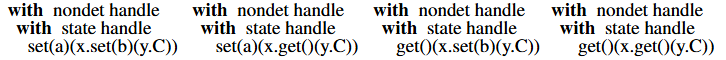
\includegraphics[width=1\textwidth]{localStateHandlerComp.png}

\caption{Standard state laws remain valid under local state, as all state operations are resolved within each branch rather than between them.}
\label{fig:local-state-laws}
\end{figure}


\subsubsection{Impermanence} 
The specification below advises that a process's local state should be lost when the process is destroyed.

\begin{tcolorbox}[colback=gray!10, colframe=gray!60, sharp corners, boxrule=0.5pt, title={POSIX Base Specifications, Issue 7, p.554}]
Memory mappings that were created in the process shall be unmapped before the process
 is destroyed.
 \end{tcolorbox}
 
We can draw a direct correspondence between our \lstinline{exit} operation and the \lstinline{fail} operation $\varnothing$ in \textit{backtrackable state} shown in Tang and Schrijvers paper. The identities below show how state is lost after failure: 

\[
\textbf{put-right-identity}: \quad \texttt{put}\;s \gg \varnothing = \varnothing
\]
\vspace{-1em}
\[
\textbf{get-right-identity}: \quad \texttt{get}\; \gg \varnothing = \varnothing
\]

The placement of the state handler inside the nondeterminism handler ensures that state is scoped to each branch individually, and when a computation fails, its state is no longer stored. The return clause also displays this property as it simply returns a value and does not resume the continuation, thereby losing all variable bindings and its associated state. The get-right-identity proof is shown below, see appendice \ref{set-fail-idempotency} for the \textit{put-right-identity} proof.

\vspace{1em}
{\large{\textbf{Proof of Exit as a Get-Right-Identity}}}

\normalsize



\begin{longtable}{@{}l@{}}
\textbf{with } nondet \textbf{ handle} \\
\quad \textbf{with } state \textbf{ handle} \\
\quad\quad \textbf{with } status \textbf{ handle} \\
\quad\quad\quad get()(x. Exit()(y. C)) \\

\quad$\equiv$ (12) \\
\textbf{with } nondet \textbf{ handle} \\
\quad \textbf{with } state \textbf{ handle} \\
\quad\quad get()(x. \textbf{with } status \textbf{ handle } Exit(v)(y. C)) \\

\quad$\equiv$ (11) \\
\textbf{with } nondet \textbf{ handle} \\
\quad fun s $\rightarrow$ (k\ s)\ s\ [fun x $\rightarrow$ \textbf{with } state, status \textbf{ handle } Exit(v)(y. C) / k] \\

\quad$\equiv$ (subst) \\
\textbf{with } nondet \textbf{ handle} \\
\quad fun s $\rightarrow$ (fun x $\rightarrow$ \textbf{with } state, status \textbf{ handle } Exit(v)(y. C)\ s)\ s \\

\quad$\equiv$ (8) \\
\textbf{with } nondet \textbf{ handle} \\
\quad fun s $\rightarrow$ \textbf{with } state, status \textbf{ handle } Exit(v)(y. C[s/x])\ s \\

\quad$\equiv$ (11) \\
\textbf{with } nondet \textbf{ handle} \\
\quad fun s $\rightarrow$ \textbf{with } state \textbf{ handle } n \\
\quad\quad [v/n,\ fun y $\rightarrow$ \textbf{with } status \textbf{ handle } C / k] 
\\ \quad$\equiv$ (subst) \\
\textbf{with } nondet \textbf{ handle} \\
\quad fun s $\rightarrow$ \textbf{with } state \textbf{ handle } v \\
\end{longtable}



\subsubsection{State Inheritance} 
The specification below advises that when a process forks the state in the parent should be copied for the child.
\begin{tcolorbox}[colback=gray!10, colframe=gray!60, sharp corners, boxrule=0.5pt, title={POSIX Base Specifications, Issue 7, p.897}]
Memory mappings created in the parent shall be retained in the child process
\end{tcolorbox}
 This ensures that both processes start from an identical state from which they may then proceed independently. Tang and Schrijvers  show how their \textit{backtrackable state} monad displays state distribution across nondeterministic choice \cite{tang2025high} :


\begin{figure}[H]  % Use [H] to force exact placement, or [htbp] for flexible
  \centering
  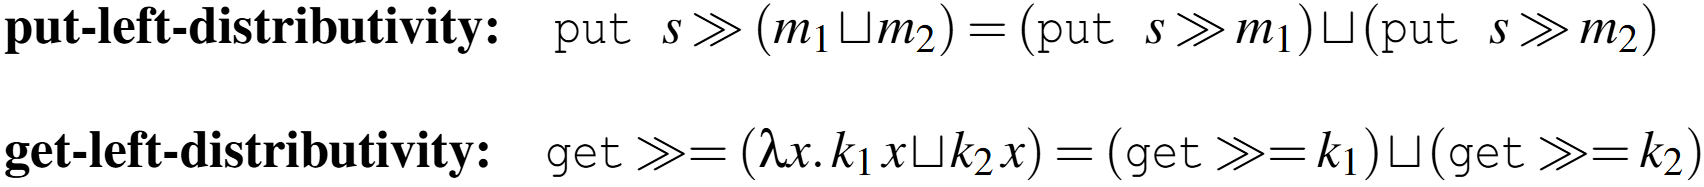
\includegraphics[width=0.9\textwidth]{distributivity.png}  % Adjust width & filename
  
\end{figure}

In line with the above properties, I can demonstrate that my handlers allow state operations to distribute over forking, following the inheritance functionality prescribed in the Unix specification. The get-left-distributivity proof is shown below, see appendice \ref{set-distributivity-over-forking} for the \textit{put-left-distributivity} proof.


{\large{\textbf{Proof - \textit{Get} Distributing Over \textit{Fork}}}}

\begin{longtable}{@{}l@{}}
\textbf{with} nondet \textbf{handle} \\ \quad
\textbf{with} state \textbf{handle} \\
\quad\quad get()(x.Fork()(y.C) \\
\quad$\equiv$ (11) \\
\textbf{with} nondet \textbf{handle} \\ \quad
fun s $\rightarrow$ (k\ s)\ s \ [fun x $\rightarrow$ \textbf{with } state handle Fork()(y.C)/k] \\
\quad$\equiv$ (subst) \\
\textbf{with} nondet \textbf{handle} \\ \quad

fun s $\rightarrow$ (fun x $\rightarrow$ \textbf{with } state handle Fork()(y.C)\ s)\ s \\
\quad$\equiv$ (8) \\
\textbf{with} nondet \textbf{handle} \\ \quad
fun s $\rightarrow$ \textbf{with } state handle Fork()(y.C)[s/x] \\
\quad$\equiv$ (12) \\
\textbf{with} nondet \textbf{handle} \\ \quad

fun s $\rightarrow$ Fork()(y.\ \textbf{with } state handle C[s/x])\ s \\
\quad$\equiv$ (11) \\
fun s $\rightarrow$ \textbf{resume } True \texttt{ ++ } \textbf{resume } False\ [fun y $\rightarrow$ \textbf{with } nondet, state handle C[s/x]] \\
\quad$\equiv$ (subst) \\
fun s $\rightarrow$ 
\quad\quad fun y $\rightarrow$ \textbf{with } nondet, state handle C[s/x]\ True \\
\quad\quad\quad\quad\quad\texttt{ ++} 
 fun y $\rightarrow$ \textbf{with } nondet, state handle C[s/x]\ False \\
\quad$\equiv$ (8) \\
fun s $\rightarrow$ \quad \textbf{with } nondet, state handle C[s/x,\ True/y] \\
\quad\quad\quad\quad \texttt{ ++} 
 \textbf{with } nondet, state handle C[s/x,\ False/y] \\
\end{longtable}






\subsection{Unix Specifications: Global State }

\begin{tcolorbox}[colback=gray!10, colframe=gray!60, sharp corners, boxrule=0.5pt, title={POSIX Base Specifications, Issue 7, p.2316}]
 This volume of POSIX.1-2008 does not specify the behaviour of concurrent writes to a regular file |
 from multiple threads, except that each write is atomic (see Section 2.9.7, onpage 522). |
 Applications should use some form of concurrency control.
\end{tcolorbox}

The term \textit{global state} refers to any memory or system resources that are shared across processes and includes the file system and other kernel-managed structures that persist independently of any single process. Since {state} is potentially modifiable by other concurrently running processes, a change made in one process can affect the behaviour of others. The Unix specifications acknowledges this concurrency problem and deals with it by delegating it to the application level. This topic will be discussed in more detail later in this chapter. 

Since execution ordering depends on the dynamic runtime state of the scheduler, algebraic reasoning is inapplicable in this scenario. 

Tang and Schrijvers also describe this problem when trying to represent global state using monads. They point out that while global state and nondeterminism can each be given a monadic structure, their composition does not form a monad. This is because state updates persist across nondeterministic branches, breaking the law of associativity and the law of identity. The composition of {nondeterminism} and {state} fails to maintain the property of right-distributivity of {nondeterminism}.


Tang and Schrijver's describe one possible global state law, the \textit{put-or} law: 
\[
\textbf{put-or:} \quad (put\ s \gg m) \oplus n = put\ s \gg (m \oplus n) 
\]

However, this another example of the equational theory being too strong to hold in a practical implementation. This law is valid in an {operational semantics} where state updates are evaluated from left to right, but in Unix systems, the order in which a scheduler's policy will run the processes cannot be assumed.


The limits of algebraic reasoning for global state evaluation are shown below. In this example a computation is evaluated until it can not be evaluated any further, because after this point the scheduler must determine the execution order.

\vspace{1em}
{\large \textbf{Example of Global State Evaluation}}
\begin{longtable}{@{}l@{}}
\textbf{with } state \textbf{ handle} \\
\quad \textbf{with } nondet \textbf{ handle} \\
\quad\quad Fork()(p.\textbf{if } p \textbf{ then } set(x)(a.C\textsubscript{1}) \textbf{ else } set(y)(b.C\textsubscript{2})) \\
\quad$\equiv$ (11) \\
 
\textbf{with } state \textbf{ handle} \\
\quad \textbf{resume } True \text{ ++ } \textbf{resume } False \\
\quad [()/v,\ \text{fun } r $\rightarrow$ \textbf{with } nondet \textbf{ handle if } r \textbf{ then } set(x)(a.C1) \textbf{ else } set(y)(b.C2)] \\

\quad$\equiv$ (\text{subst}) \\
\textbf{with } state \textbf{ handle} \\
\quad fun r $\rightarrow$ \textbf{with } nondet \textbf{ handle if } r \textbf{ then } set(x)(a.C1) \textbf{ else } set(y)(b.C2)\ True \\
\quad ++ \\
\quad fun r $\rightarrow$ \textbf{with } nondet \textbf{ handle if } r \textbf{ then } set(x)(a.C1) \textbf{ else } set(y)(b.C2)\ False \\

\quad$\equiv$ (8) \\
\textbf{with } state \textbf{ handle} \\
\quad \textbf{with } nondet \textbf{ handle if } True \textbf{ then } set(x)(a.C1) \textbf{ else } set(y)(b.C2) \\
\quad ++ \\
\quad \textbf{with } nondet \textbf{ handle if } False \textbf{ then } set(x)(a.C1) \textbf{ else } set(y)(b.C2) \\

\quad$\equiv$ (5,6) \\
\textbf{with } state \textbf{ handle} \\
\quad \textbf{with } nondet \textbf{ handle } set(x)(a.C1) \\
\quad ++ \\
\quad \textbf{with } nondet \textbf{ handle } set(y)(b.C2) \\

\quad$\equiv$ (12) \\
\textbf{with } state \textbf{ handle} \\
\quad set(x)(a.\textbf{with } nondet \textbf{ handle } C1) \\
\quad ++ \\
\quad set(y)(b.\textbf{with } nondet \textbf{ handle } C2) \\
\end{longtable}


It will be seen that this creates a nondeterministic outcome, as the order in which the scheduler chooses to run these branches will affect the final state of the system. 



\section{Process Synchronisation}
\label{process-synchronisation}

Initially, I had hoped that \textit{process synchronisation primitives} would offer a rich avenue for algebraic reasoning; however, this soon proved to be impossible due the inherent inability to model the scheduler algebraically.

To illustrate the necessity of synchronisation primitives, one must first understand the limitations of the basic scheduler. The scheduler provides process interleaving, but it does not provide an ability to order the execution of processes, i.e. it is "nondeterministic". 

Nondeterminism is problematic because, as already demonstrated, many of the \textit{effects} are non-commutative, meaning that the order of their execution can influence their observable behaviour. This can give rise to a \textit{race condition} - a scenario where two or more concurrent processes attempt to access or modify shared state simultaneously, with the final result depending on the exact timing of these interleavings.

Hillerström mitigates this problem by introducing a more complex scheduler that can handle \lstinline{wait} operations. These allow a process to suspend further execution until the process it is waiting on finishes. However, this is still not enough to ensure correct write ordering, as other processes could still potentially alter, i.e. corrupt, the resource whilst the original process is suspended.  

To maintain flexibility around process interleaving and to guarantee write ordering, we introduce a new feature, a \textit{mutex}, which can be combined with the \lstinline{wait} operation. A \textit{mutex} is a locking mechanism used to ensure that only one process can access a shared resource at a time.


By combining these synchronisation primitives we can:
\begin{enumerate}
    \item Lock a resource to prevent other processes interfering with it.
    \item Enforce correct process orderings using \lstinline{wait} operations.
\end{enumerate}


However, despite my best attempts, reasoning about these partial ordering guarantees proved difficult. Unlike other features in the system, the schedulers semantics rely on mutable structures (specifically, the state of the process queue) which fall outside the scope of static algebraic equivalences.

Schedulers are notoriously difficult to reason about formally. \textit{Pretnar}, in \textit{The Logic and Handling of Algebraic Effects} \cite{Pretnar:2010}, highlights the difficulty of representing the synchronisation operator with effect handlers. This operator takes two computations as arguments and is used to model concurrent execution. The issue stems from the recursive nature of both its parameters: each argument is a computation that can diverge further independently of one another, so the recursive proof cannot rely on either side remaining fixed. Without a clearly decreasing argument, primitive recursion is impossible, making traditional inductive reasoning inapplicable.

\section{Reasoning Conclusions}
\label{reasoning-conclusion}
In this chapter I showed how algebraic equivalences can be used to reason about the behaviour of effect handlers. I began by reasoning about the properties of my. \lstinline{status} handler, showing that exceptions only hold the absorption property, and discussed how many of the rules that held in an isolated setting break down under composition with this handler. 

I then examined a simplified model of state, which enabled reasoning about the environment variables in my system. I tried to extend this method to a more complex state model, reasoning about the file system; however, this approach quickly became impractical, as the equivalences grew too complex to manage.


From here, I discussed the forking operation and considered the properties of nondeterminism in our system, demonstrating how they differ from the notion of nondeterminism found in abstract equational theories.

In the penultimate section of this chapter, I explored two models of state, local and global. These are determined by the composition order of the {nondeterminism} and {state} handlers and how explained that global state corresponds to shared file system state, while local state corresponds to process-local state. For both models of state, I verified that they possessed algebraic properties, fulfilling the Unix specifications.

As mentioned previously, it is notoriously difficult  to reason about properties which depend on the scheduler. Consequently, reasoning about any forms of process synchronisation to provide partial ordering and safe writing guarantees was not possible.

In conclusion, this chapter can be summarised by the following observations:
\begin{itemize}
    \item Algebraic reasoning proved effective for verifying the correctness of simple handlers. However, more complex handlers without associated equational theories often proved too difficult to reason about in practice.
    \item There are limitations to what can be reasoned about with algebraic equivalences - vital features like the scheduler are outwith their applicable scope.
\end{itemize}


\chapter{Conclusions}

\section{Unix Implementation in Koka}
In this project I have implemented the \textit{Tiny Unix} system described by Hillerström. I implemented exception handling, a basic I/O scheme, user functionality, a basic serial file system, piping, and two methods of process scheduling. I successfully achieved my first goal by demonstrating that it is possible to simulate a Unix-like system in Koka in a concise and modular manner, despite the complex challenges this posed.

\textbf{Future Work: } The Koka implementation could be extended by including the features described in section \ref{process-synchronisation}. Currently, the system cannot guarantee a correct write order unless it is done sequentially, i.e. within a single process and without interrupts, defeating the purpose of a time-sharing system. The addition of \textit{mutexes} with \lstinline{wait} operations would address this problem and provide correct interleaved writing.

\section{Reasoning}
Although I was able to verify that some features of my Unix implementation comply with the rules set out in the Unix Specifications, I was unable to formally prove the correctness  of all features using algebraic equivalences, due to the challenges discussed in section \ref{reasoning-conclusion}.

\textbf{Future Work: } This project could be expanded by exploring the techniques of automated reasoning outlined in McLaughlin's PhD thesis, \textit{Relational Reasoning for Effects and Handlers
} \cite{McLaughlin2020}. In particular, this approach could be especially useful in verifying my implementation of piping. Pretnars paper \textit{An Introduction to
Algebraic Effects and Handlers} \cite{pretnar_introduction_2015} he introduces a set of operational rules which could be used to provide similar proofs. 

% \bibliographystyle{plain}
\bibliographystyle{plain}
\bibliography{mybibfile}


% You may delete everything from \appendix up to \end{document} if you don't need it.
\appendix

\chapter{Proofs} 

\section{Simplified State} \label{full-simplified-single-cell-state-proof}

\subsection{Idempotence of Set}
Performing consecutive \lstinline{set} operations retains only the final update, as each invocation completely overwrites the current state:
\[
\begin{aligned}
    &\mathsf{\textbf{with}} \; \mathsf{state} \; \mathsf{\textbf{handle}} \\
    &\quad \operatorname{set} \; a \; (x. \operatorname{set} \; b \; (y. C)) \\
    &\equiv \\
    &\mathsf{\textbf{with}} \; \mathsf{state} \; \mathsf{\textbf{handle}} \\
    &\quad \operatorname{set} \; b \; (y. C)
\end{aligned}
\]

\underline{Left Hand Side}

\begin{longtable}{@{}l@{}}
\quad$\equiv$ (11) \\
\text{fun }$\_$ \rightarrow (k\ ())\ s\ [a/s,\ \text{fun } x \rightarrow \textbf{with } state \textbf{handle } set(b)(y.C)/k] \\
\quad$\equiv$ (subst) \\
\text{fun }$\_$ \rightarrow ((\text{fun } x \rightarrow \textbf{with } state \textbf{handle } set(b)(y.C))\ ())\ a \\
\quad$\equiv$ (8) \\
\text{fun }$\_$ \rightarrow (\textbf{with } state \textbf{handle } set(b)(y.C))\ a \\
\quad$\equiv$ (11) \\
\text{fun }$\_$ \rightarrow (\text{fun }\_ \rightarrow (k\ ())\ s\ [b/s,\ \text{fun } y \rightarrow \textbf{with } state \textbf{handle } C/k])\ a \\
\quad$\equiv$ (subst) \\
\text{fun }\_ \rightarrow (\text{fun }\_ \rightarrow (\text{fun } y \rightarrow \textbf{with } state \textbf{handle } C)\ ())\ b)\ a \\
\quad$\equiv$ (8) \\
\text{fun }$\_$ \rightarrow (\text{fun }\_ \rightarrow (\textbf{with } state \textbf{handle } C)\ b)\ a \\
\quad$\equiv$ (application) \\
\text{fun }$\_$ \rightarrow (\textbf{with } state \textbf{handle } C)\ b \\
\end{longtable}


\underline{Right Hand Side}
\[ 
\begin{array}{l}
\quad\equiv\quad (11) \\[5pt]
\text{fun }\_ \rightarrow (k\ ())\ s\ [b/s, \text{fun } y \rightarrow \text{\textbf{with} state \textbf{handle} } C/k] \\[5pt]
\quad\equiv\quad (\text{subst}) \\[5pt]
\text{fun }\_ \rightarrow ((\text{fun } y \rightarrow \text{\textbf{with} state \textbf{handle} } C)\ ())\ b \\[5pt]
\quad\equiv\quad (8) \\[5pt]
\text{fun }\_ \rightarrow (\text{\textbf{with} state \textbf{handle} } C)\ b
\end{array}
\]

LHS $\equiv$ RHS

\subsection{Idempotence of Get}
Reading the state multiple times without an intervening \lstinline{set} yields the same result each time. Repeating a get operation without modifying the state in between has no observable effect on the computation.


\[
\begin{aligned}
    &\mathsf{\textbf{with}} \; \mathsf{state} \; \mathsf{\textbf{handle}} \\
    &\quad \operatorname{get}() \left( \mathsf{x.get}() \left( y.C \right) \right) \\
    &\equiv \\
    &\mathsf{\textbf{with}} \; \mathsf{state} \; \mathsf{\textbf{handle}} \\
    &\quad \operatorname{get}() \left( x.C[x/y] \right)
\end{aligned}
\]
\underline{Left Hand Side}

\[ 
\begin{array}{l}
\quad\equiv\quad (11) \\[5pt]
\text{fun } s \rightarrow (k\ s)\ s\ [()/v, \text{fun } x \rightarrow \text{\textbf{with} state \textbf{handle} } get()(y.C)/k] \\[5pt]
\quad\equiv\quad (\text{subst}) \\[5pt]
\text{fun } s \rightarrow ((\text{fun } x \rightarrow \text{\textbf{with} state \textbf{handle} } get()(y.C))\ s)\ s \\[5pt]
\quad\equiv\quad (8) \\[5pt]
\text{fun } s \rightarrow (\text{\textbf{with} state \textbf{handle} } get()(y.C[s/x]))\ s \\[5pt]
\quad\equiv\quad (11) \\[5pt]
\text{fun } s \rightarrow ((\text{fun } s'\rightarrow (k\ s')\ s')\ [()/v, \text{fun } y\rightarrow \text{\textbf{with} state \textbf{handle}}/k])\ s \\[5pt]
\quad\equiv\quad (\text{subst}) \\[5pt]
\text{fun } s \rightarrow ((\text{fun } s' \rightarrow (( \text{fun } y \rightarrow \text{\textbf{with} state \textbf{handle} } C[s/x])\ s')\ s')\ s \\[5pt]
\quad\equiv\quad (8) \\[5pt]
\text{fun } s \rightarrow (\text{fun } s' \rightarrow (\text{\textbf{with} state \textbf{handle} } C[s/x][s'/y]s')) \\[5pt]
\quad\equiv\quad (8) \\[5pt]
\text{fun } s \rightarrow (\text{\textbf{with} state \textbf{handle} } C[s/x][s/y])\ s
\end{array}
\]



\underline{Right Hand Side}

\[ 
\begin{array}{l}
\quad\equiv\quad (11) \\[5pt]
\text{fun } s \rightarrow (k\ s)\ s\ [()/v, C[x/y]] \\[5pt]
\quad\equiv\quad (\text{subst}) \\[5pt]
\text{fun } s \rightarrow ((\text{fun } x \rightarrow \text{\textbf{with} state \textbf{handle} } C[x/y])) \\[5pt]
\quad\equiv\quad (8) \\[5pt]
\text{fun } s \rightarrow (\text{\textbf{with} state \textbf{handle} } C[x/y][s/x])\ s
\end{array}
\]

LHS $\equiv$ RHS



\subsection{Set-Then-Get}
Reading the state immediately after setting it yields the value that was just written. This property ensures that state updates are immediately observable.
\[
\begin{aligned}
    &\mathsf{\textbf{with}} \; \mathsf{state} \; \mathsf{\textbf{handle}} \\
    &\quad \operatorname{set} \; a \; (x. \operatorname{get}() \; (y. C)) \\
    &\equiv \\
    &\mathsf{\textbf{with}} \; \mathsf{state} \; \mathsf{\textbf{handle}} \\
    &\quad \operatorname{set} \; a \; (x. C[a/x])
\end{aligned}
\]

\underline{Left Hand Side}
\[ 
\begin{array}{l}
\quad\equiv\quad (11) \\[5pt]
\text{fun }\_ \rightarrow (k\ ())\ s\ [a/s, \text{fun } x \rightarrow \text{\textbf{with} state \textbf{handle} } get() (y. C)/k] \\[5pt]
\quad\equiv\quad (\text{subst}) \\[5pt]
\text{fun }\_ \rightarrow ((\text{fun } x \rightarrow \text{\textbf{with} state \textbf{handle} } get() (y. C)) ())\ a \\[5pt]
\quad\equiv\quad (8) \\[5pt]
\text{fun }\_ \rightarrow (\text{\textbf{with} state \textbf{handle} } get() (y. C))\ a \\[5pt]
\quad\equiv\quad (11) \\[5pt]
\text{fun }\_ \rightarrow (\text{fun } s' \rightarrow  (k\ s')\ s' [()/s, \text{fun } y \rightarrow \text{\textbf{with} state \textbf{handle} } C / k])\ a \\[5pt]
\quad\equiv\quad (\text{subst}) \\[5pt]
\text{fun }\_ \rightarrow ((\text{fun } s' \rightarrow ((\text{fun } y \rightarrow \text{\textbf{with} state \textbf{handle} } C)\ s' )\ s')\ a \\[5pt]
\quad\equiv\quad (\text{application}) \\[5pt]
\text{fun }\_ \rightarrow ((\text{fun } y \rightarrow \text{\textbf{with} state \textbf{handle} } C)\ a )\ a \\[5pt]
\quad\equiv\quad (8) \\[5pt]
\text{fun }\_ \rightarrow (\text{\textbf{with} state \textbf{handle} } C[a/y])\ a
\end{array}
\]

\underline{Right Hand Side}
\[ 
\begin{array}{l}
\quad\equiv\quad (11) \\[5pt]
\text{fun }\_ \rightarrow (k\ ())\ s\ [a/s, \text{fun } x \rightarrow \text{\textbf{with} state \textbf{handle} } C[a/y]/k] \\[5pt]
\quad\equiv\quad (\text{subst}) \\[5pt]
\text{fun }\_ \rightarrow ((\text{fun } x \rightarrow \text{\textbf{with} state \textbf{handle} } C[a/y]) ())\ a \\[5pt]
\quad\equiv\quad (8) \\[5pt]
\text{fun }\_ \rightarrow (\text{\textbf{with} state \textbf{handle} } C[a/y])\ a
\end{array}
\]



\subsection{Get-Then-Set}
A \lstinline{get} followed by a \lstinline{set}, updates the state with a new value whilst preserving the former state value by binding it in the continuation. 


\[
\begin{aligned}
    &\mathsf{\textbf{with}} \; \mathsf{state} \; \mathsf{\textbf{handle}} \\
    &\quad \operatorname{get}() \left( x. \operatorname{set} \; a \; (y. C) \right) \\
    &\equiv \\
    &\mathsf{\textbf{with}} \; \mathsf{state} \; \mathsf{\textbf{handle}} \\
    &\quad \operatorname{set} \; a \; (y. C[s/x])
\end{aligned}
\]

\underline{Left Hand Side}
\[ 
\begin{array}{l}
\quad\equiv\quad (11) \\[5pt]
\text{fun } s \rightarrow (k\ s)\ s\ [()/v, \text{fun } x \rightarrow \text{\textbf{with} state \textbf{handle} } set(a)(y.C)/k] \\[5pt]
\quad\equiv\quad (\text{subst}) \\[5pt]
\text{fun } s \rightarrow ((\text{fun } x \rightarrow \text{\textbf{with} state \textbf{handle} } set(a)(y.C))\ s)\ s \\[5pt]
\quad\equiv\quad (8) \\[5pt]
\text{fun } s \rightarrow (\text{\textbf{with} state \textbf{handle} } set(a)(y.C[s/x]))\ s \\[5pt]
\quad\equiv\quad (11) \\[5pt]
\text{fun } s \rightarrow ((\text{fun } \_ \rightarrow (k\ ())\ s')[a/s', \text{fun } y \rightarrow \text{\textbf{with} state \textbf{handle} } C[s/x]/k])\ s' \\[5pt]
\quad\equiv\quad (\text{subst}) \\[5pt]
\text{fun } s \rightarrow (\text{fun } \_ \rightarrow (\text{\textbf{with} state \textbf{handle} } C[s/x]) ())\ a \\[5pt]
\quad\equiv\quad (8) \\[5pt]
\text{fun } s \rightarrow (\text{\textbf{with} state \textbf{handle} } C[s/x])\ a
\end{array}
\]


\underline{Right Hand Side}
\[ 
\begin{array}{l}
\quad\equiv\quad (11) \\[5pt]
\text{fun }\_ \rightarrow (k\ ())\ s\ [a/s, \text{fun } y \rightarrow \text{\textbf{with} state \textbf{handle} } C[s/x]/k] \\[5pt]
\quad\equiv\quad (\text{subst}) \\[5pt]
\text{fun }\_ \rightarrow (\text{fun } y \rightarrow \text{\textbf{with} state \textbf{handle} } C[s/x]) ()\ a \\[5pt]
\quad\equiv\quad (8) \\[5pt]
\text{fun }\_ \rightarrow (\text{\textbf{with} state \textbf{handle} } C[s/x]\ a)
\end{array}
\]
LHS $\equiv$ RHS

\section{Environment Variable Proofs} \label{environment-variable-proofs}

\subsection{Su-Su}

\renewcommand{\arraystretch}{1}
\begin{longtable}{@{}l@{}}
{sessionmgr} $\langle \mathit{user}_i,\; \textbf{Su}(\mathit{user}_j)(x.\;\textbf{Su}(\mathit{user}_k)(y.C)) \rangle$ \\[5pt]

\hspace*{2em} $\equiv$ (apply) \\[5pt]
\textbf{with }\text{env} $\langle \mathit{user}_i \rangle$ \textbf{handle} \\ 
\hspace*{2em} \textbf{with session handle} \textbf{Su}$(\mathit{user}_j)(x.\;\textbf{Su}(\mathit{user}_k)(y.C))$ \\[5pt]

\hspace*{2em} $\equiv$ (11) \\[5pt]
\textbf{with }\text{env} $\langle \mathit{user}_i \rangle$ \textbf{handle} \\ 
\hspace*{2em} \text{env} $\langle \mathit{user}',\; m \rangle\; [\mathit{user}_j/\mathit{user}',\; \text{fun } x \rightarrow \textbf{with session handle}\; \textbf{Su}(\mathit{user}_k)(y.C)/m]$ \\[5pt]

\hspace*{2em} $\equiv$ (subst) \\[5pt]
\textbf{with }\text{env} $\langle \mathit{user}_i \rangle$ \textbf{handle} \\ 
\hspace*{2em} \textbf{with }\text{env} $\langle \mathit{user}_j \rangle$ \textbf{handle} \\ 
\hspace*{4em} \textbf{with session handle} \textbf{Su}$(\mathit{user}_k)(y.C)$ \\[5pt]

\hspace*{2em} $\equiv$ (11) \\[5pt]
\textbf{with }\text{env} $\langle \mathit{user}_i \rangle$ \textbf{handle} \\ 
\hspace*{2em} \textbf{with }\text{env} $\langle \mathit{user}_j \rangle$ \textbf{handle} \\ 
\hspace*{4em} \text{env} $\langle \mathit{user}',\; m \rangle\; [\mathit{user}_k/\mathit{user}',\; \text{fun } y \rightarrow \textbf{with session handle}\; C/m]$ \\[5pt]

\hspace*{2em} $\equiv$ (subst) \\[5pt]
\textbf{with }\text{env} $\langle \mathit{user}_i \rangle$ \textbf{handle} \\ 
\hspace*{2em} \textbf{with }\text{env} $\langle \mathit{user}_j \rangle$ \textbf{handle} \\ 
\hspace*{4em} \textbf{with }\text{env} $\langle \mathit{user}_k \rangle$ \textbf{handle} \\ 
\hspace*{6em} $C$
\end{longtable}





\subsection{Su-Ask}

\begin{longtable}{@{}l@{}}
\textbf{sessionmgr}$\langle \text{user}_i \rangle$ \ \textbf{Su(}\text{user}_j\textbf{)}(x.\ \textbf{whoami}()) \\

\quad$\equiv$\quad (apply) \\
\textbf{with } env$\langle \text{user}_i \rangle$ \textbf{handle} \\
\quad \textbf{with } session \textbf{handle } Su(\text{user}_j)(x.\ \textbf{whoami}()(y. C)) \\

\quad$\equiv$\quad (11) \\
\textbf{with } env$\langle \text{user}_i \rangle$ \textbf{handle} \\
\quad env$\langle \text{user}',\ \text{resume} \rangle$ \ [\text{user}_j/\text{user}',\ fun x $\rightarrow$ \textbf{with } session \textbf{handle } \textbf{whoami}()(y. C) / resume] \\

\quad$\equiv$\quad (subst) \\
\textbf{with } env$\langle \text{user}_i \rangle$ \textbf{handle} \\
\quad env$\langle \text{user}_j,\ fun x \rightarrow \textbf{with } session \textbf{handle } \textbf{whoami}()(y. C) \rangle$ \\

\quad$\equiv$\quad (11) \\
\textbf{with } env$\langle \text{user}_i \rangle$ \textbf{handle} \\
\quad \textbf{with } env$\langle \text{user}_j \rangle$ \textbf{handle} \\
\quad\quad \textbf{with } session \textbf{handle } \textbf{whoami}()(y. C) \\

\quad$\equiv$\quad (12) \\
\textbf{with } env$\langle \text{user}_i \rangle$ \textbf{handle} \\
\quad \textbf{with } env$\langle \text{user}_j \rangle$ \textbf{handle } \textbf{whoami}()(y.\ \textbf{with } session \textbf{handle } C) \\

\quad$\equiv$\quad (11) \\
\textbf{with } env$\langle \text{user}_i \rangle$ \textbf{handle} \\
\quad \textbf{case user \{} \\
\quad\quad \text{user}_1\ $\rightarrow$ \textbf{resume } "user_1" \\
\quad\quad \cdots \\
\quad\quad \text{user}_n\ $\rightarrow$ \textbf{resume } "user_n" \\
\quad \} \ [()/v,\ fun y $\rightarrow$ \textbf{with } env$\langle \text{user}_j \rangle$, session \textbf{handle } C / resume] \\

\quad$\equiv$\quad (subst) \\
\textbf{with } env$\langle \text{user}_i \rangle$ \textbf{handle } fun y $\rightarrow$ \textbf{with } env$\langle \text{user}_j \rangle$, session \textbf{handle } C \ "user$_j$" \\

\quad$\equiv$\quad (8) \\
\textbf{with } env$\langle \text{user}_i \rangle$ \textbf{handle } \textbf{with } env$\langle \text{user}_j \rangle$, session \textbf{handle } C["user_j"/y] \\
\end{longtable}



\subsection{Ask-Ask}
\[
\begin{array}{l}
\text{sessionmgr}⟨\text{user}_i⟩\ \text{whoami}()(x.\ \text{whoami}()(y.\ C)) \\[5pt]

\quad\equiv\quad (\text{apply}) \\[5pt]
\textbf{with } \text{env}⟨\text{user}_i⟩\ \textbf{handle} \\
\quad \textbf{with } \text{session}\ \textbf{handle}\ \text{whoami}()(x.\ \text{whoami}()(y.\ C)) \\[5pt]

\quad\equiv\quad (12) \\[5pt]
\textbf{with } \text{env}⟨\text{user}_i⟩\ \textbf{handle}\ \text{whoami}()(x.\ \textbf{with } \text{session}\ \textbf{handle}\ \text{whoami}()(y.\ C)) \\[5pt]

\quad\equiv\quad (11) \\[5pt]
\text{case user \{} \\
\quad \text{user}_1\ \rightarrow\ \text{resume } "user_1" \\
\quad \cdots \\
\quad \text{user}_n\ \rightarrow\ \text{resume } "user_n" \\
\text{\}}\ [()/v,\ \text{fun } x\ \rightarrow\ \textbf{with } \text{env}⟨\text{user}_j⟩, \text{session}\ \textbf{handle } \text{whoami}()(y.\ C)/\text{resume}] \\[5pt]

\quad\equiv\quad (\text{subst}) \\[5pt]
\text{fun } x\ \rightarrow\ \textbf{with } \text{env}⟨\text{user}_j⟩, \text{session}\ \textbf{handle } C\ "user_j" \\[5pt]

\quad\equiv\quad (8) \\[5pt]
\textbf{with } \text{env}⟨\text{user}_j⟩\ \textbf{handle} \\
\quad \textbf{with } \text{session}\ \textbf{handle }\ \text{whoami}()(y.\ C["user_j"/x]) \\[5pt]

\quad\equiv\quad (12) \\[5pt]
\textbf{with } \text{env}⟨\text{user}_j⟩\ \textbf{handle}\ \text{whoami}()(y.\ \textbf{with } \text{session}\ \textbf{handle } C["user_j"/x]) \\[5pt]

\quad\equiv\quad (11) \\[5pt]
\text{case user \{} \\
\quad \text{user}_1\ \rightarrow\ \text{resume } "user_1" \\
\quad \cdots \\
\quad \text{user}_n\ \rightarrow\ \text{resume } "user_n" \\
\text{\}}\ [()/v,\ \text{fun } y\ \rightarrow\ \textbf{with } \text{env}⟨\text{user}_j⟩, \text{session}\ \textbf{handle } C["user_j"/x] / \text{resume}] \\[5pt]

\quad\equiv\quad (\text{subst}) \\[5pt]
\text{fun } y\ \rightarrow\ \textbf{with } \text{env}⟨\text{user}_j⟩, \text{session}\ \textbf{handle } C["user_j"/x,\ "user_j"/y] \\[5pt]

\quad\equiv\quad (8) \\[5pt]
\textbf{with } \text{env}⟨\text{user}_j⟩\ \textbf{handle} \\
\quad \textbf{with } \text{session}\ \textbf{handle } C["user_j"/x,\ "user_j"/y] \\
\end{array}
\]

\subsection{Ask-Su}

\[
\begin{array}{l}
\text{sessionmgr}⟨\text{user}_i⟩\ \text{whoami}()(x.\ \text{Su}(\text{user}_j)(y.\ C)) \\[5pt]

\quad\equiv\quad (\text{apply}) \\[5pt]
\textbf{with } \text{env}⟨\text{user}_i⟩\ \textbf{handle} \\
\quad \textbf{with } \text{session}\ \textbf{handle }\ \text{whoami}()(x.\ \text{Su}(\text{user}_j)(y.\ C)) \\[5pt]

\quad\equiv\quad (12) \\[5pt]
\textbf{with } \text{env}⟨\text{user}_i⟩\ \textbf{handle} \\
\quad \text{whoami}()(x.\ \textbf{with } \text{session}\ \textbf{handle }\ \text{Su}(\text{user}_j)(y.\ C)) \\[5pt]

\quad\equiv\quad (11) \\[5pt]
\textbf{with } \text{env}⟨\text{user}_i⟩\ \textbf{handle} \\
\quad \text{case user \{} \\
\quad\quad \text{user}_1\ \rightarrow\ \text{resume } "user_1" \\
\quad\quad \cdots \\
\quad\quad \text{user}_n\ \rightarrow\ \text{resume } "user_n" \\
\quad\} \\
\quad [()/v,\ \text{fun } x\ \rightarrow\ \textbf{with } \text{session}\ \textbf{handle }\ \text{Su}(\text{user}_j)(y.\ C) / \text{resume}] \\[5pt]

\quad\equiv\quad (\text{subst}) \\[5pt]
\textbf{with } \text{env}⟨\text{user}_i⟩\ \textbf{handle} \\
\quad \text{fun } x\ \rightarrow\ \textbf{with } \text{session}\ \textbf{handle }\ \text{Su}(\text{user}_j)(y.\ C)\ "user_j" \\[5pt]

\quad\equiv\quad (8) \\[5pt]
\textbf{with } \text{env}⟨\text{user}_i⟩\ \textbf{handle} \\
\quad \textbf{with } \text{session}\ \textbf{handle }\ \text{Su}(\text{user}_j)(y.\ C["user_j"/x]) \\[5pt]

\quad\equiv\quad (11) \\[5pt]
\textbf{with } \text{env}⟨\text{user}_i⟩\ \textbf{handle} \\
\quad \text{env}⟨\text{user}', m⟩\ [\text{user}_j/\text{user}',\ \text{fun } y\ \rightarrow\ \textbf{with } \text{session}\ \textbf{handle } C["user_j"/x]] \\[5pt]

\quad\equiv\quad (\text{subst}) \\[5pt]
\textbf{with } \text{env}⟨\text{user}_i⟩\ \textbf{handle} \\
\quad \textbf{with } \text{env}⟨\text{user}_j⟩\ \textbf{handle} \\
\quad\quad \textbf{with } \text{session}\ \textbf{handle } C["user_j"/x] \\
\end{array}
\]


\section{Set-Fail Idempotency} \label{set-fail-idempotency}
\begin{longtable}{@{}l@{}}
\textbf{with } nondet \textbf{ handle} \\
\quad \textbf{with } state \textbf{ handle} \\
\quad\quad \textbf{with } status \textbf{ handle} \\
\\
\quad$\equiv$ (12) \\
\textbf{with } nondet \textbf{ handle} \\
\quad \textbf{with } state \textbf{ handle} \\
\quad\quad set(a)(x. \textbf{with } status \textbf{ handle } Exit(v)(y. C)) \\
\\
\quad$\equiv$ (11) \\
\textbf{with } nondet \textbf{ handle} \\
\quad fun \_ $\rightarrow$ (k ())\ s\ [a/s,\ fun x $\rightarrow$ \textbf{with } state, status \textbf{ handle } Exit(v)(y. C) / k] \\
\\
\quad$\equiv$ (subst) \\
\textbf{with } nondet \textbf{ handle} \\
\quad fun \_ $\rightarrow$ (fun x $\rightarrow$ \textbf{with } state, status \textbf{ handle } Exit(v)(y. C))()\ a \\
\\
\quad$\equiv$ (8) \\
\textbf{with } nondet \textbf{ handle} \\
\quad fun \_ $\rightarrow$ \textbf{with } state, status \textbf{ handle } Exit(v)(y. C)\ a \\
\\
\quad$\equiv$ (11) \\
\textbf{with } nondet \textbf{ handle} \\
\quad fun \_ $\rightarrow$ \textbf{with } state, status \textbf{ handle } n \\
\quad\quad [v/n,\ fun y $\rightarrow$ \textbf{with } status \textbf{ handle } C / k]\ a \\
\\
\quad$\equiv$ (subst) \\
\textbf{with } nondet \textbf{ handle} \\
\quad fun \_ $\rightarrow$ \textbf{with } state, status \textbf{ handle } v\ a \\
\end{longtable}




\section{Set Distributivity over Forking} \label{set-distributivity-over-forking}
\begin{longtable}{@{}l@{}}
\textbf{with } nondet \textbf{ handle} \\
\quad \textbf{with } state \textbf{ handle} \\
\quad\quad set(a)(x. Fork()(y. C)) \\
\\
\quad$\equiv$ (11) \\
\textbf{with } nondet \textbf{ handle} \\
\quad fun \_ $\rightarrow$ (k())\ s\ [a/s,\ fun x $\rightarrow$ \textbf{with } state \textbf{ handle } Fork()(y. C)] \\
\\
\quad$\equiv$ (subst) \\
\textbf{with } nondet \textbf{ handle} \\
\quad fun \_ $\rightarrow$ (fun x $\rightarrow$ \textbf{with } state \textbf{ handle } Fork()(y. C))()\ a \\
\\
\quad$\equiv$ (apply) \\
\textbf{with } nondet \textbf{ handle} \\
\quad fun \_ $\rightarrow$ \textbf{with } state \textbf{ handle } Fork()(y. C)\ a \\
\\
\quad$\equiv$ (12) \\
\textbf{with } nondet \textbf{ handle} \\
\quad fun \_ $\rightarrow$ Fork()(y. \textbf{with } state \textbf{ handle } C)\ a \\
\\
\quad$\equiv$ (11) \\
fun \_ $\rightarrow$ \textbf{resume } True \texttt{ ++ } \textbf{resume } False \\
\quad [fun y $\rightarrow$ \textbf{with } nondet, state \textbf{ handle } C / resume]\ a \\
\\
\quad$\equiv$ (subst) \\
fun \_ $\rightarrow$ \\
\quad fun y $\rightarrow$ \textbf{with } nondet, state \textbf{ handle } C\ True \\
\quad\quad \texttt{++} \quad \quad \quad \quad \quad \quad \quad \quad \quad \quad \quad \quad \quad \quad \quad \quad \quad a\\
\quad fun y $\rightarrow$ \textbf{with } nondet, state \textbf{ handle } C\ False \\
\end{longtable}


\section{Koka Implementation}
\label{koka-implementation}

\begin{lstlisting}
module unix
import std/core/console

fun main()
  with bio
  echo("Douglas Torrance, 2025")

// =========================================
// Section 3.1 - Status
// =========================================

effect exit
  ctl exit(n : int) : a

fun status(action : () -> <exit|e> a) : e int
  with handler 
    return(x) -> 0
    ctl exit(code) code
  action()

// =========================================
// Section 3.2 - Basic IO
// =========================================

alias filedesc = int
val stdout = 0

effect bio
  // writeBio a string to a file descriptor
  fun writeBio( fd : filedesc, s : string ) : ()

fun bio( action : () -> <bio|e> a ) : e (a,string)
  var buf := ""    
  with handler
    return (x) -> (x, buf)
    fun writeBio(fd, s) -> { buf := buf ++ s }
  action()

fun echo( s : string ) : bio ()
  writeBio(stdout,s)

// =========================================
// Section 3.3 - User Environment
// =========================================

type user
  Root
  Alice
  Bob

effect su
  ctl su( u : user ) : ()

effect whoami
  fun whoami() : string

fun env( user : user, action : () -> <whoami|e> a ) : e a
  with fun whoami() 
    match user
      Root  -> "root"
      Alice -> "alice"
      Bob   -> "bob"
  action()

fun sessionmgr( u : user, action : () -> <su,whoami|e> a ) : e a
  with env(u)
  with ctl su( u' : user )
         mask<whoami>
           with env(u')
           resume(())
  action()

// =========================================
// Section 3.4 - Multi-Process System
// =========================================

// 3.4.1 - Forking

effect fork
  ctl fork() : bool     

fun forking( action : () -> <fork|e> a ) : e list<a>
  with handler
    return(x) [x]
    ctl fork() resume(True) ++ resume(False)
  action()

// 3.4.2 - Scheduling
type pstate<e,a>
  Done(result : a)
  Paused(resumption : () -> e pstate<e,a> )

effect interrupt
  ctl interrupt() : ()

fun reify-process(action : () -> <interrupt|e> a) : e pstate<e,a> 
  with handler  
    return(x) -> Done(x)
    ctl interrupt() -> Paused(fn() resume(()))
  action()

fun scheduler( pstates : list<pstate<<fork,div|e>,a>> ) : <div|e> list<a>
  fun schedule( todos : list<pstate<<fork,div|e>,a>>, done : list<a> ) : <div|e> list<a>
    match todos
      Nil -> done
      Cons(Done(x),ps') -> schedule(ps', Cons(x,done))
      Cons(Paused(m),ps') ->
        val ps = forking( m )
        schedule( ps' ++ ps, done )
  schedule(pstates,[])

fun timeshare( action : () -> <fork,interrupt,div|e> a ) : <div|e> list<a>
  val p = Paused( fn() reify-process(action) )
  scheduler([p])

fun interrupt-writeBio( action : () -> <bio,interrupt|e> a ) : <bio,interrupt|e> a
  with override fun writeBio(fd,s) { interrupt(); writeBio(fd,s) }
  action()

// =========================================
// Section 3.5 - Basic Serial File System
// =========================================

type directory 
  Directory
    d_list : list<(string, int)>

type dataRegion 
  DataRegion
    dr : list<(int, string)>

type iNode
  INode
    no : int
    loc : int

type iList 
  IList
    il : list<(int, iNode)>  

struct fileSystem
  dir   : directory
  ilist : iList
  dreg  : dataRegion
  dnext : int
  inext : int

val fs0 : fileSystem =
  FileSystem (
    Directory([("stdout", 0)]),
    IList([(0, INode ( 1, loc = 0 ))]),
    DataRegion([(0, "")]),
    1,
    1
  )

// Section 3.5.1 - File Reading and Writing

effect fileRW
  ctl read( ino : int ) : option<string>
  ctl write( ino : int, s : string ) : ()

fun fread( ino : int, fs : fileSystem ) : <div,fail|e> string
  val inode = lookupINode(ino, fs.ilist)
  lookupDataRegion(inode.loc, fs.dreg)
  

fun fwrite( ino : int, contents : string, fs : fileSystem ) : <div,fail|e> fileSystem
  match fs
    FileSystem(dir, ilist, dreg, dnext, inext) -> 
      val inode  = lookupINode(ino, ilist)
      val oldstr = lookupDataRegion(inode.loc, dreg)  
      val newstr = oldstr ++ contents  
      val newdr  = modifyDataRegion(inode.loc, newstr, dreg)  
      FileSystem(dir, ilist, newdr, dnext, inext)

effect fail
  ctl fail() : a

fun withDefault<a>(default: a, m: () -> <fail|e>a) : e a
  with handler
    return(x) -> x
    ctl fail() -> default
  m()

fun fileRW<a>(m: () -> <fileRW,div,state<fileSystem>|e>a) : <state<fileSystem>,div|e>  a 
  with handler
    fun read(ino) 
      val cs = withDefault(None, fn() -> Some(fread(ino, get())))
      cs
    fun write(ino, cs) 
      withDefault((), fn() 
          val fsys  = get()
          val fsys' = fwrite(ino, cs, fsys)
          put(fsys')
          ()
      )
  m()

type option<t>
  Some { value : t }
  None

effect state<a> 
  ctl get() : a
  ctl put(x: a) : ()

// Section 3.5.2 - File Creation and File Opening

effect fileCO
  ctl create( fname : string ) : option<int>
  ctl open( fname : string ) : option<int>

fun fopen(fname: string, fs : fileSystem) 
  match fs.dir 
    Directory(d_list) ->
      match d_list 
        Nil        -> fail()  
        Cons((k, v), rest) ->
          if k == fname then v
          else lookupDirectory(fname, Directory(rest))
      
fun fcreate(fname: string, fs: fileSystem) : <div,fail> (int, fileSystem) 
  if has(fname, fs.dir) then 
    val ino = fopen(fname, fs)  
    val inode = lookupINode(ino, fs.ilist)  
    val dreg' = modifyDataRegion(inode.loc, "", fs.dreg)  
    (ino, FileSystem(fs.dir, fs.ilist, dreg', fs.dnext, fs.inext))  
  
  else 
    val loc = fs.dnext  
    val dreg' = DataRegion(Cons((loc, ""), fs.dreg.dr))  
    val ino = fs.inext  
    val inode = INode(loc, 1)  
    val ilist' = IList(Cons((ino, inode) , fs.ilist.il))  
    val dir' = Directory(Cons((fname, ino), fs.dir.d_list))  
    val fs' = FileSystem(dir', ilist', dreg', fs.dnext + 1, fs.inext + 1)  
    (ino, fs')

fun has<a, b>(key: string, xs: directory) : <div> bool
  withDefault(False, fn() {
    val disc = lookupDirectory(key, xs)  
    True  
  })

fun fileCreateOpen<a>(action : () -> <fileCO, div, state<fileSystem>|e> a) : <state<fileSystem>,div|e> a
  with handler 
    return(x) -> x
    ctl create(name) 
      val maybeIno = withDefault(None, fn() {
        val fs0 = get()
        val (ino,fs1) = fcreate(name, fs0)
        put(fs1)
        Some(ino)
      })
      resume(maybeIno)
    
    ctl open(name) 
      val maybeIno = withDefault(None, fn() {
        val fs0 = get()
        val ino = fopen(name, fs0)
        Some(ino)
      })
      resume(maybeIno)
  action()

// Section 3.5.3 - File Linking

effect fileLU
  fun link(src: string, tgt : string) :()

fun flink(src : string, dest : string, fs : fileSystem) : <div,fail> fileSystem 
  if has(dest, fs.dir) then
    fail()  
  else 
    val ino = lookupDirectory(src, fs.dir)
    val dir' = Directory(Cons((dest, ino), fs.dir.d_list))
    val inode = lookupINode(ino, fs.ilist)
    val inode' = INode(inode.no, inode.loc + 1)
    val ilist' = modifyINode(ino, inode', fs.ilist)

    FileSystem(dir', ilist', fs.dreg, fs.dnext, fs.inext)

pub fun fileLU(action: () -> <fileLU, div, state<fileSystem>|e> a): <state<fileSystem>, div|e> a
  with handler
    fun link(src, tgt)
      with withDefault(())
      val fs = flink(src, tgt, get())
      put(fs)

  action() 
  
// =========================================
// Section 3.6 - Piping
// =========================================

effect produce<b>
  ctl produce(x : b) : ()   // yield a value of type b

effect consume<b>
  ctl consume() : b         // await/ask for a value of type b

fun pipe(p : () -> <produce<b>, div|e> a, c : () -> <consume<b>, div|e> a): <div|e> a
    with raw ctl consume()
      copipe(p, fn(x) rcontext.resume-shallow(x) )
    c()

fun copipe(p : () -> <produce<b>, div|e> a, c : b -> <consume<b>, div|e> a): <div|e> a
    with raw ctl produce(y)
      pipe(fn() rcontext.resume-shallow(()), fn() c(y))
    p()


// =========================================
// Section 3.7 - Process Synchronisation
// =========================================

effect co
  ctl ufork() : int
  ctl wait(pid: int): ()
  ctl uinterrupt() :()
  
alias proc<a,e> = sstate<a,e> -> e list<(int, a)>

rec type spstate<a,e>
  Ready
    r : proc<a,e>
  Blocked 
    pid :int 
    proc:proc<a,e>

type sstate<a,e> 
  Sstate     
    q : list<(int, spstate<a,e>)>
    done  : list<(int,a)>
    pid   : int
    pnext : int

pub fun runState(init:b, action: () -> <div, state<b>|e> a): <div|e> (b,a)
  var curr := init
  with handler
    return(x)   (curr,x)
    fun get()   curr
    fun put(x)  curr := x
  action() 

fun runNext(st: sstate<a,<div|e>> ) : <div|e> list<(int,a)> 
  match st.q
    Nil -> st.done
    Cons((bpid, Blocked(pid', proc)), ps) -> 
      val newQ = ps ++ [(bpid, Blocked(pid', proc))]
      val newsState =  Sstate (q = newQ, done = st.done, pid = st.pid, pnext = st.pnext)
      runNext(newsState) 
    Cons((rpid, Ready(res)), ps) -> 
      val newState =  Sstate (q = ps, done = st.done, pid = rpid, pnext = st.pnext)
      res(newState)

fun scheduler2<a,e>(state:sstate<a,<div|e>>, action:() -> <co,div|e> a): <div|e> list<(int,a)>
  val h = 
    with handler
      return(x)
        fn(st)
          val done' = st.done ++ [(st.pid, x)]
          runNext(Sstate(q=st.q, done=done', pid = st.pid, pnext=st.pnext))
        
      ctl uinterrupt()
        fn(st)
          val resumption = fn(st') resume( () ) (st')
          val q' = st.q ++ [(st.pid, Ready(resumption))]
          runNext(Sstate(q=q',done=st.done, pid=st.pid,pnext=st.pnext))
        
      ctl wait(pid')
        fn(st)
          val resumption = fn(st') resume(()) (st')
          val q' =  if hasPid(pid', st.q) then 
                      st.q ++ [(st.pid, Blocked(pid', resumption))] 
                    else 
                      st.q ++ [(st.pid, Ready(resumption))]
          runNext(Sstate(q=q',done=st.done, pid=st.pid,pnext=st.pnext))
        
      ctl ufork()
        fn(st)
          val resumption = fn(st') resume(0)(st')
          val pid' = st.pnext
          val q' = st.q ++ [(pid', Ready(resumption))]
          resume(pid')(Sstate(q=q', done=state.done, pid = st.pnext, pnext=pid'+1))
      
    action()
  h(state)

pub fun timeshare2(action: () -> <co,div|e> a): <div|e> list<(int,a)>
  with scheduler2(Sstate( [], [], 1, 2))
  action()

// =====================================
// Helper Functions
// =====================================

fun hasPid<a>(pid : int, xs : list<(int, spstate<a,e>)>) : bool 
  match xs
    Nil -> False
    Cons((pid1, _), rest) ->
      if pid1 == pid then True else hasPid(pid, rest)


fun lookupDirectory(key : string, xs : directory) : <div, fail|e> int
  match xs
    Directory (d_list) ->
      match d_list
        Nil -> fail()  
        Cons((k, v), rest) ->
          if k == key
          then v
          else lookupDirectory(key, Directory ( d_list = rest ))

fun lookupINode(key : int, xs : iList) : <div, fail|e> iNode
  match xs
    IList(il) ->
      match il
        Nil -> fail()  
        Cons((k, v), rest) -> 
          if k == key
          then v
          else lookupINode(key, IList(rest))  

fun lookupDataRegion(key : int, xs : dataRegion) : <div, fail|e> string
  match xs
    DataRegion(dr) ->  
      match dr
        Nil -> fail()  
        Cons((k, v), rest) ->
          if k == key
          then v
          else lookupDataRegion(key, DataRegion(rest))  

fun modifyDirectory(key : string, value : int, xs : directory) : directory
  match xs
    Directory(d_list) ->
      Directory(modifyListDirectory(key, value, d_list))

fun modifyListDirectory(key : string, value : int, xs : list<(string, int)>) : list<(string, int)>
  match xs
    Nil -> [(key, value)]  // If key is not found, insert new entry
    Cons((k, v), rest) ->
      if k == key
      then Cons((key, value), rest)  // Replace existing value
      else Cons((k, v), modifyListDirectory(key, value, rest))  // Recurse

fun modifyINode(key : int, value : iNode, xs : iList) : iList
  match xs
    IList(il) ->
      IList(modifyListINode(key, value, il))

fun modifyListINode(key : int, value : iNode, xs : list<(int, iNode)>) : list<(int, iNode)>
  match xs
    Nil -> [(key, value)]  // Insert new entry if key is not found
    Cons((k, v), rest) ->
      if k == key
      then Cons((key, value), rest)  // Replace existing value
      else Cons((k, v), modifyListINode(key, value, rest))  // Recurse

fun modifyDataRegion(key : int, value : string, xs : dataRegion) : dataRegion
  match xs
    DataRegion(dr) ->
      DataRegion(modifyListDataRegion(key, value, dr))

fun modifyListDataRegion(key : int, value : string, xs : list<(int, string)>) : list<(int, string)>
  match xs
    Nil -> [(key, value)]  // Insert new entry if key is not found
    Cons((k, v), rest) ->
      if k == key
      then Cons((key, value), rest)  // Replace existing value
      else Cons((k, v), modifyListDataRegion(key, value, rest))  // Recurse

pub fun fileIO(action: () -> <fileRW, fileCO, fileLU, state<fileSystem>,div|e> a): <state<fileSystem>, div|e> a
  with fileRW
  with fileCreateOpen
  with fileLU
  action()





\end{lstlisting}

\end{document}
